% The Norns III paper: a packer that keeps the HDL's structure, a known-optimum yardstick and the leak it
% found. Rewritten 2026-10-28 as hypothesis -> experiment -> verdict (docs/paper/hypotheses.md is the register).
% IEEEtran conference class; compiles with pdfLaTeX (Overleaf) and BibTeX. Style and figures follow the Odin III
% paper (shared TikZ palette, IMAGE/odin3-tikz-styles.tex). Numbers trace to committed files (comments at the number).
\documentclass[conference]{IEEEtran}

\usepackage{cite}
\usepackage{amsmath}
\usepackage{graphicx}
\usepackage{booktabs}
\usepackage{array}
\usepackage{url}
\usepackage{listings}
\usepackage{tikz}
\usetikzlibrary{positioning,fit,arrows.meta,shapes.geometric,backgrounds,calc,matrix}

\graphicspath{{IMAGE/}}
% Shared TikZ styles for the Odin III paper figures (IMAGE/fig_*.tex).
% Needs: \usepackage{tikz} and
%   \usetikzlibrary{positioning,fit,arrows.meta,shapes.geometric,backgrounds,calc,matrix}
% loaded first (odin3.tex and IMAGE/figures.tex both do). Input this file once, in the preamble.
%
% Palette: the greens and browns of a tree and its greenery, with black for Odin's raven as the
% strong ink. Green = ColorBrewer "Greens", brown = a warm earth ramp. Text is dark on the light
% fills and white only on the dark browns and the black.

% ---- colours ------------------------------------------------------------------------------
\definecolor{o3ink}{HTML}{111111}      % text and arrows: the raven's black
\definecolor{o3sub}{HTML}{4E342E}      % secondary text (sub-project tags, notes): dark brown
\definecolor{o3grn9}{HTML}{00441B}
\definecolor{o3grn8}{HTML}{006D2C}
\definecolor{o3grn7}{HTML}{238B45}
\definecolor{o3grn5}{HTML}{74C476}
\definecolor{o3grn4}{HTML}{A1D99B}
\definecolor{o3grn3}{HTML}{C7E9C0}
\definecolor{o3grn2}{HTML}{E5F5E0}
\definecolor{o3grn1}{HTML}{F7FCF5}
\definecolor{o3brn9}{HTML}{3E2723}     % root system, dark brown (white text only)
\definecolor{o3brn8}{HTML}{5D4037}
\definecolor{o3brn7}{HTML}{4E342E}
\definecolor{o3brn6}{HTML}{6D4C41}     % trunk
\definecolor{o3brn5}{HTML}{8D6E63}
\definecolor{o3brn4}{HTML}{C9B6A4}     % branches, lighter brown
\definecolor{o3brn3}{HTML}{E0D3C6}
\definecolor{o3brn2}{HTML}{F1E9DF}
\definecolor{o3brn1}{HTML}{F8F4EE}

% ---- text helpers -------------------------------------------------------------------------
% A second, smaller line in a node: \odinsub{2C}.
\newcommand{\odinsub}[1]{{\scriptsize\color{o3sub}#1}}
% Code names inside figures (the paper's \code is not defined in the standalone build).
\newcommand{\odintt}[1]{\texttt{#1}}

% Scale a figure down only if it is wider than #1 (it never scales up). Each figure is drawn
% at its print size, so this is a safety net; a scaled figure writes "ODINFIT" to the log.
\newsavebox{\odinfigbox}
\newcommand{\odinfit}[2]{%
  \sbox{\odinfigbox}{\ignorespaces#2\unskip}%
  \ifdim\wd\odinfigbox>#1\relax
    \typeout{ODINFIT: figure scaled from \the\wd\odinfigbox\space to \the#1}%
    \resizebox{#1}{!}{\usebox{\odinfigbox}}%
  \else
    \usebox{\odinfigbox}%
  \fi}

% ---- TikZ styles --------------------------------------------------------------------------
\tikzset{
  % every figure
  odin/.style={font=\footnotesize, color=o3ink, line join=round,
               >={Stealth[length=3.4pt, width=2.8pt]},
               % node text breaks the same way in any class: no hyphens, loose lines rather than overfull
               execute at begin node={\hyphenpenalty=10000\exhyphenpenalty=10000%
                 \tolerance=9999\emergencystretch=10pt}},
  % shapes
  box/.style={draw, rectangle, rounded corners=1.6pt, align=center, line width=0.55pt,
              inner xsep=2.5pt, inner ysep=2pt, minimum height=6.5mm},
  store/.style={draw, cylinder, shape border rotate=90, aspect=0.16, align=center,
                line width=0.55pt, inner xsep=2pt, inner ysep=1pt, minimum height=8mm},
  plain/.style={align=center, inner sep=1pt},
  % neutral fills for structure figures
  neutral/.style={fill=o3brn2, draw=o3brn6, solid},
  light/.style={fill=o3grn1, draw=o3grn7, solid},
  external/.style={fill=o3brn2, draw=o3brn6, dash pattern=on 3pt off 1.2pt on 0.6pt off 1.2pt},
  emph/.style={line width=1.3pt},
  % grouped regions, drawn on the background layer
  region/.style={draw=o3brn4, fill=o3brn1, rounded corners=3pt, line width=0.5pt,
                 inner sep=4pt},
  bluregion/.style={draw=o3grn3, fill=o3grn1, rounded corners=3pt, line width=0.5pt,
                    inner sep=4pt},
  regionlabel/.style={font=\scriptsize\bfseries, color=o3brn7, inner sep=1.5pt},
  % arrows
  flow/.style={->, line width=0.55pt, draw=o3ink},
  ref/.style={->, line width=0.5pt, draw=o3grn8, dash pattern=on 2.4pt off 1.4pt},
  edgelabel/.style={font=\scriptsize, color=o3sub, inner sep=1pt, fill=white},
  % records: a header row and field rows, built with \matrix (see fig_ir_model.tex)
  record/.style={matrix of nodes, ampersand replacement=\&, row sep=-\pgflinewidth,
                 inner sep=0pt, nodes={draw=o3brn6, line width=0.5pt, fill=white,
                 font=\scriptsize, anchor=center, align=left, inner xsep=2.5pt,
                 inner ysep=1.2pt, minimum height=4.4mm}},
  rechead/.style={fill=o3grn3, font=\scriptsize\bfseries, align=center},
}

% \odinrecord{<name>}{<matrix options: position, nodes={text width=...}>}{<header>}{<rows>}
% A record (struct) as a one-column matrix: a header cell, then one cell per field, rows
% separated by \\ and ended by \\. Cells are <name>-<row>-1, so edges can leave from a field.
\newcommand{\odinrecord}[4]{%
  \matrix[record, #2] (#1) {|[rechead]| #3 \\ #4};}


\newcommand{\code}[1]{\texttt{#1}}
% Run-in heading (IEEEtran's \paragraph is numbered and adds a colon).
\newcommand{\pp}[1]{\par\vspace{3pt}\noindent\textit{#1}\ }
% Glossary: run-in terms, no hanging label column.
\newenvironment{gloss}{\begin{list}{}{\setlength{\leftmargin}{0pt}\setlength{\labelwidth}{0pt}\setlength{\labelsep}{0pt}\setlength{\itemindent}{0pt}\setlength{\itemsep}{1pt}\setlength{\parsep}{0pt}\setlength{\topsep}{2pt}\renewcommand{\makelabel}[1]{\textbf{##1}\hspace{0.5em}}}}{\end{list}}
% A visible marker for numbers not yet measured.
\newcommand{\todo}[1]{\textbf{[TODO: #1]}}
\lstset{basicstyle=\ttfamily\scriptsize, columns=fullflexible, keepspaces=true,
        frame=single, framesep=2pt, xleftmargin=3pt, xrightmargin=3pt,
        aboveskip=4pt, belowskip=4pt}

\title{The Norns~III: Does Keeping the HDL's Structure Help FPGA Packing?\\
A Known-Optimum Yardstick and Negative Results}

\author{\IEEEauthorblockN{Peter Jamieson}
\IEEEauthorblockA{Electrical and Computer Engineering, Miami University\\
Oxford, OH, USA\\
jamiespa@miamioh.edu}}

\begin{document}
\maketitle

\begin{abstract}
Before an FPGA design is placed on a chip, the grouping the designer wrote down in the source is mostly lost, and the packer that groups logic into tiles uses only local information about the circuit. This paper asks whether keeping that grouping, or any other cheap change to packing and placement, buys a deployable gain in speed, wire or area, and closes with a negative answer. We measured the room first. A yardstick of designs built so that the best grouping is known shows that the standard packer uses 22\% more wire than the known grouping over all topologies and 49\% more on meshes and trees, and on 33 real designs made into known-optimum yardsticks it needs 1.108 times the proven lower bound on CLBs and 1.265 times the wire (delay inconclusive). Its decision log puts 60\% of the CLB gap in one kind of pick: an atom of another cluster taken while the right one was queued. We then tried every change we could define from local, answer-free information. An HDL-aware packer first showed a 0.902 wirelength ratio, which was a leak (the input equalled the answer); with realistic registers it used 65\% to 150\% more wire. Refreshing criticality while packing, a seed rule, a two-hop gain term, Schabas-style spare room and duplication after placement each gave a geomean speed change between $-2.1\%$ and $+0.7\%$ with wins and losses nearly even (best: 17 wins, 14 losses, 4 ties), and none beat noise; the two apparent speed gains were selections on the number they were scored on. A true seed oracle that uses the answer key improves wire by 2.8\% and CLBs by 1.2\% but not speed, and rebuilds only 25.5\% of the known clusters. The reading is that modern APPack is near what local information reaches, and that the 2003 results of Schabas and Brown do not replicate on VTR~9. Threats: the yardstick is optimal for area and cut, not timing; one architecture and 35 designs. Of 77 register hypotheses, 15 are useful, 10 possibly good, 27 inconclusive and 25 dismissed; 11 further rows are measurements and ten ideas are untested and parked.
\end{abstract}

\begin{IEEEkeywords}
FPGA packing, placement, provenance, known-optimum benchmarks, VTR
\end{IEEEkeywords}

\section{Introduction}
\label{sec:intro}

An FPGA is a chip made of many small programmable logic blocks joined by programmable wires; a design is loaded onto it by setting those parts. A designer writes the design in a hardware description language (HDL), and a chain of CAD programs turns that text into a pattern on the chip. Two steps of the chain decide most of the result. Packing groups small pieces of logic into tile-sized groups, and placement decides where on the chip each group sits. Packing and placement see the design as a long list of gates and wires. The grouping the designer wrote down (this register, that adder, that block of the source) is mostly gone by then.

This paper asks one question: does keeping the designer's grouping, or any other cheap change to packing and placement, make the result better, and how can we find out honestly? The answer is a closed negative one. We answer it with hypotheses. Each hypothesis is stated in plain language, an experiment is run, and the experiment either confirms it or does not. Ideas that the experiments confirm are in the main text; ideas that failed are one line in the research log (Appendix~\ref{sec:log}). The work ends here, with a negative-results paper whose lasting contribution is a set of designs with a known best grouping, because the experiments that followed it found no change that beats noise.

\pp{The paper in four sentences.} First, we measured how much room a packer has by building designs whose best grouping is known; the standard packer leaves room in tile count and wire. Second, we tried every change we could define from information the packer can see (the designer's registers, refreshed timing weights, a starting-atom rule, a two-hop gain term, spare room in critical groups, duplication after placement); none gave a speed, wire or tile-count gain that stands apart from noise (Table~\ref{tab:tried}). Third, the changes that looked like gains were a flaw in the benchmark and two selections on the scored number. Fourth, a modern packer is near what local, answer-free information reaches, and the 2003 gains of Schabas and Brown do not replicate on VTR~9 (Section~\ref{sec:summary}).

\pp{What good means.} A real design is judged on three things at once: the chip area it needs (low), its speed (high) and its power (low). We measure area and speed. Power is not measured in any experiment of this paper. Speed means the slowest path of the design and also the paths nearly as slow, because speeding up the slowest path alone only promotes the next one (Section~\ref{sec:method}).

\pp{The data behind it.} M\'{\i}mir~III is the dataset this work feeds. Every piece of the circuit carries a record of the HDL text it came from. M\'{\i}mir stores that record beside where each piece was placed and how fast its paths are, so the data can show \emph{why} things ended up where they did, and not only where. Section~\ref{sec:mimir} says what M\'{\i}mir holds today and what it lacks.

\pp{The innovations, in plain English.}
\begin{enumerate}
\item \textbf{A packer that knows the grouping.} It is a copy of the standard open-source packer with a bonus for putting pieces of one HDL register or bus into the same tile (Section~\ref{sec:i-packer}).
\item \textbf{A yardstick with a known best grouping.} We build designs out of blocks that each exactly fill one tile, so the best tile grouping is known, and measure how far a packer is from it (Section~\ref{sec:i-yardstick}).
\item \textbf{A leak found by the yardstick.} The first test of the new packer showed a gain of nearly ten percent in wire used. The yardstick showed that the gain came from an input file that already contained the answer: a leak. With groupings that do not mirror the answer, the packer used more wire at every setting we tried (Section~\ref{sec:i-leak}). We state this plainly because it is a lesson about method: a gain that exists only when the tool is handed the solution is not a gain.
\item \textbf{A count of what the standard packer keeps together on slow paths} (Section~\ref{sec:i-census}).
\item \textbf{A negative baseline.} Starting placement from the designer's grouping instead of the tool's own start did not help (Section~\ref{sec:i-seed}).
\item \textbf{A second yardstick from real designs.} The synthetic yardstick is too regular: its wiring hardly changes with the size of the region around a block, as real wiring does (Section~\ref{sec:i-rent}). So we edit real designs until their grouping is the known best (Section~\ref{sec:i-yardstick-real}).
\item \textbf{Where the greedy packer goes wrong.} We measure the connections the packer treats as nearly the slowest, show that most of its picks from them are for connections that are not slow in the finished design, and keep a catalogue of the HDL patterns for which the pick goes wrong (Sections~\ref{sec:e-heap} and~\ref{sec:e-pick}).
\end{enumerate}

\pp{Contributions.} Each is an innovation with the hypotheses that the experiments settled; the headline is the CAD one (mean percent win and wins, losses and ties, in the order speed, wire, area), then the register verdict. (1) The standard packer scatters the source's registers across tiles (H8), and the new packer keeps them together without using more tiles (H9a; mechanism checks, not end results), all \textsc{useful}. (2) The yardstick is exact (H24, H27, H29--H31: \textsc{useful}) and shows room: the standard packer uses 22\% more wire than the known grouping over all topologies and 49\% more on meshes and trees (H25/H19, H32: \textsc{useful}); on 33 real designs it needs 1.108 times the proven lower bound on tiles and 1.265 times the wire of the known grouping, with the delay \textsc{inconclusive} (H38: \textsc{useful}). (3) The new packer's gain exists only when the HDL registers equal the blocks (H33, H36, H35: \textsc{useful}, an upper bound and a harm finding); with realistic registers it uses 65\% to 150\% more wire and 33\% to 41\% more delay (H22$'$: \textsc{dismissed}). (4) Where the standard packer goes wrong is measured: 60\% of its tile-count gap is a pick of an atom of another known group while the right atom was queued (Q-N2), and no feature computable from the circuit alone ranks the right atom well once the construction is removed (Q-N3). (5) The deployable changes all failed to beat noise. Speed: refreshing the timing weights $-0.5\%$ (H-refresh, \textsc{inconclusive}), a two-hop gain term $+0.7\%$ with 17 wins, 14 losses, 4 ties (\textsc{inconclusive}), spare room $-1.4\%$ to $-2.1\%$ and duplication $-0.5\%$ and $-0.4\%$ (\textsc{dismissed} or \textsc{inconclusive}); each costs or gains about one percent of wire and, for spare room, 11\% to 17\% more tiles (Table~\ref{tab:tried}). (6) A starting-atom oracle that uses the answer key improves wire by 2.8\% (25 wins, 8 losses) and the tile count by 1.2\% (23, 6, 4 ties) but not speed ($-0.7\%$; 13 wins, 20 losses), and rebuilds only 25.5\% of the known groups (Q-N1b). (7) A sweep of tool options gives eight \textsc{possibly good} area and speed effects (Section~\ref{sec:e10}), and the packer's idea of which connections are slowest is stale for 81\% of its picks (HP-1, a measurement). In total the research log has 88 rows: 15 \textsc{useful}, 10 \textsc{possibly good}, 27 \textsc{inconclusive}, 25 \textsc{dismissed}, and eleven measurements; ten untested ideas, listed in Section~\ref{sec:future}, sit beside them.


\section{Background}
\label{sec:background}

This section defines every term of the paper once, in dependency order, so that no term is used before its definition. The basic definitions follow the order and the wording of the FPGA and CAD background chapters of two University of Toronto theses of the same research line~\cite{jamiesonthesis,luu2014thesis}: the soft logic fabric and the basic logic element, the three CAD stages that follow synthesis, and (from Luu) timing criticality. The terms that are the paper's own come after them.

\subsection{Glossary}
\label{sec:glossary}

\begin{gloss}
% Each definition is on one line; check_terms.py reads these lines (docs/paper/terms.md).
\item[FPGA] A chip made of many small programmable logic blocks joined by programmable wires; a design is loaded onto it~\cite{jamiesonthesis}.
\item[netlist] A list of the logic gates of a design and the wires between them~\cite{jamiesonthesis}.
\item[HDL] Hardware description language: the Verilog text a designer writes.
\item[LUT] Look-up table: the small memory that implements any logic function of a few inputs~\cite{jamiesonthesis,luu2014thesis}.
\item[$K$] The number of inputs of a LUT; here $K=6$.
\item[BLE] Basic logic element: one LUT with its flip-flop~\cite{jamiesonthesis,luu2014thesis}.
\item[cluster] A set of netlist blocks that are meant to belong together; a clustering is a partition of the netlist into clusters.
\item[CLB] Configurable logic block: a group of 10 BLEs placed as one unit (a logic block or soft logic cluster tile in the theses).
\item[module] One HDL module, the unit of the design hierarchy.
\item[provenance] The record kept on every netlist object of which HDL text, and which module, it came from.
\item[word] A group of netlist blocks that are the bits of one HDL vector (a register, an adder or a bus).
\item[io-word] A word made from a top-level input or output bus, extended inward to the logic next to it.
\item[placement] The choice of which site on the chip each block occupies; a placer makes it~\cite{jamiesonthesis}.
\item[routing] The choice of which wire segments connect the placed blocks; the router makes it~\cite{jamiesonthesis}.
\item[VPR] The place-and-route program of the VTR flow~\cite{rose2012vtr,luu2014vtr7,murray2020vtr8}.
\item[wirelength] The total length of the routed wires of a design (WL); lower means less routing area and usually less delay.
\item[critical path] The slowest register-to-register path of a design; it sets the clock speed.
\item[CPD] Critical-path delay: the delay of the critical path, in nanoseconds.
\item[slack] How much earlier than required a signal arrives; negative slack means the clock is too fast. VPR normalises slack by the CPD~\cite{luu2014thesis}.
\item[near-critical] A path (or connection) whose delay is within a stated fraction of the CPD; criticality is $1-\text{slack}/\text{CPD}$~\cite{luu2014thesis}, and VPR~9 relaxes it per timing constraint~\cite{wainberg2015relaxed}.
\item[channel width] The number of routing tracks per channel; a smaller routable width needs less wire area.
\item[packing] The step that groups LUTs and flip-flops into CLBs before placement; VPR's packer is AAPack~\cite{jamiesonthesis,luu2014thesis}.
\item[simulated annealing] A placement search that accepts worse moves at a falling temperature, to escape bad layouts.
\item[analytic placement] A placement computed by solving a smooth wirelength model; VPR's starting point for the anneal~\cite{murray2020vtr8}.
\item[affinity packing] The Norns packer: a copy of VPR's packer with a bonus $\beta$ for adding atoms of the same word or module to a CLB (the affinity file names the group of each atom).
\item[purity] The share of a CLB's labelled atoms that carry its most common word (or module), atom-weighted over CLBs.
\item[split factor] How many CLBs a word spans, divided by the fewest CLBs that could hold it; 1.0 is best.
\item[known-optimum yardstick] A design built from blocks that each fill exactly one CLB, so the intended clustering is known by construction; it is an optimum for CLB count only and not a proven best placement.
\item[alignment] How closely the HDL words match the blocks of a yardstick design: 1 means each word is one block, 0 means each word holds about ten blocks' bits.
\item[leak] A gain that exists only because the input file (the word file) already equals the answer (the block partition).
\item[pairing class] The class of a pair of atoms in one CLB: series-critical, series-noncritical, shared-input, orthogonal or filler.
\item[seed] A placement file given to VPR to start the anneal from, instead of its own start; soft seeds may be left by the anneal and hard seeds are floorplan regions it must keep.
\item[Urd] The provenance seed: its clusters are the HDL modules.
\item[Verdandi] The recovered seed: clusters found from the flat netlist alone (Loki~III L2: Louvain, spectral, affinity propagation, $k$-means)~\cite{loki3}.
\item[quotient layout] A die layout of clusters: contract each cluster to a node, weight edges by cut nets, lay the small graph out and scale it to the die.
\item[scale $S$] The anneal's start temperature as a multiple of VPR's own automatic estimate.
\item[crossover] The largest tested scale $S$ at which a seeded cold start still routes shorter than an unseeded run.
\item[retention] The fraction of a seed's CLBs still inside the seed cluster's region when the anneal ends.
\item[hindsight clustering] The stock clustering with atoms moved or swapped between neighbouring CLBs according to where the best stock placement put them.
\item[flat-placement file] VPR's one-line-per-atom placement file (\code{--read\_flat\_place}), through which an outside placer enters VPR.
\item[nextpnr] An open-source FPGA placer with an analytic mode (HeAP) and an annealing mode (SA)~\cite{gort2012heap,shah2019nextpnr}.
\item[reread control] The control that reads VPR's own final placement back into the default flow.
\item[rule H0] Adders, multipliers, RAMs and pads are fixed at VPR's analytic positions for the external placers.
\item[run record] A \code{mimir-run.json} written for each VPR or nextpnr run: commands, tool commits, parameters with their source, hashes.
\item[geomean ratio] The geometric mean over designs of variant over reference; below 1 favours the variant for a lower-is-better metric.
\item[sign test] An exact two-sided test on how many designs improve; ties are left out.
\item[Wilcoxon test] A rank test of the paired per-design differences (one-sided where the text says so).
\item[Holm adjustment] The correction of p-values for several simultaneous tests.
\item[bootstrap interval] A confidence interval from resampling the designs.
\item[verdict rule] The numeric rule that maps a result to supported, not supported or inconclusive.
\end{gloss}

Three more terms are used as plain words and need no entry: \emph{area} is the LUT count, the CLB count, the die grid and the channel width; \emph{speed} is the CPD and the near-critical statistics; \emph{power} is not measured (Section~\ref{sec:metrics}).

\subsection{Concepts}

The flow runs in this order. The front end reads the HDL and writes a netlist (here Odin~III, with the provenance record on every object). Packing groups the netlist into CLBs. Placement puts the CLBs and the fixed blocks on the die: VPR starts from an analytic placement and refines it by simulated annealing. Routing connects the placed blocks, and timing analysis reports slack and the CPD~\cite{rose2012vtr,luu2014vtr7,murray2020vtr8}. The designer's grouping is a property of the HDL. It can be lost at each step: the front end may drop the register boundaries, packing mixes registers in a CLB for connectivity, and the anneal moves CLBs freely.

Two earlier lines of work connect to this question. Gharibian et al.\ recovered system-level structure from flat netlists and showed that it correlates with placement locality~\cite{gharibian2010finding,gharibian2013analyzing,gharibian2014identifying}. Cong, Romesis and Xie built placement problems with known optima to measure how far placers are from them~\cite{Cong03tpeko}; our yardstick follows that idea for packing. RLPlace improves the anneal itself with directed moves and checkpointing~\cite{elgammal2022rlplace}; we leave the anneal as it is.

\subsection{Where the Norns sits in the suite}

Figure~\ref{fig:yggdrasil} places The Norns~III in the suite. Yggdrasil~III is drawn as a tree. Odin~III is the trunk, and the provenance record that the packer uses comes from its one IR. The Norns~III is a side branch, a tool and experiment for placement with provenance, next to Loki~III (reverse engineering, whose L2 clusterings are the recovered seeds), Leman~Russ~III and Verdandi~III. It runs Odin~III and VPR as programs and changes neither. M\'{\i}mir~III, the circuit knowledge base, hangs from the canopy as the fruit, and the Norns' run records are among what it stores. Urdarbrunnr, the well of FPGA CAD and its views (VTR and VPR, nextpnr, DREAMPlaceFPGA, OpenPARF), feeds The Norns~III.

\begin{figure*}[tp]
\centering
\odinfit{\textwidth}{% Yggdrasil III drawn as a tree. Roots (dark brown) at the bottom: what Odin III reads and writes, and the
% tools it links to. The trunk (brown) is Odin III, its steps running DOWN from parse to the roots. A small
% forest of mini trees on the right holds the oracles, to compare against. The canopy (green oval) is the
% tree-top: Wyrd III, Bifrost III (the arrow to Midgard III) and Midgard III (verilogTown). Loki III,
% Leman Russ III, The Norns III and Verdandi III are side branches off the trunk, tools and experiments.
% Mimir III is the fruit: three round fruits hang from the canopy on short stems; it is the harvest of
% the trunk and the branches (Odin III, The Norns III, Loki III feed it with every run).
% Three deep roots reach three wells (Mimisbrunnr, Urdarbrunnr, Hvergelmir): the outside work the suite
% draws on; the oracle trees root into Hvergelmir too. No status; the GitHub links are in the caption.
\definecolor{o3wel1}{HTML}{E8F1F8}     % well water
\definecolor{o3wel8}{HTML}{3B6E99}     % well rim
\begin{tikzpicture}[odin, node distance=3mm,
  leaf/.style={ellipse, draw=o3grn8, fill=o3grn1, align=center, line width=0.6pt, inner xsep=1pt,
               inner ysep=1pt, minimum width=15mm, minimum height=8.5mm, font=\scriptsize},
  tip/.style={rectangle, rounded corners=3pt, draw=o3brn9, fill=o3brn3, align=center, line width=0.6pt, inner xsep=1pt,
              inner ysep=1pt, minimum height=7mm, font=\scriptsize},
  limb/.style={line width=8pt, draw=o3brn5, line cap=round},
  limbin/.style={line width=5.8pt, draw=o3brn4, line cap=round},
  rootl/.style={line width=3.4pt, draw=o3brn9, line cap=round},
  rootin/.style={line width=1.6pt, draw=o3brn7, line cap=round},
  stp/.style={font=\scriptsize\bfseries, text=white, inner sep=0pt, align=center},
  mini/.style={ellipse, draw=o3grn8, fill=o3grn3, line width=0.5pt, align=center, inner sep=0pt,
               minimum width=17mm, minimum height=12mm, font=\scriptsize}]
  % ---- deep roots to the three wells (drawn first, behind everything): the outside work the suite
  % ---- draws on. Hvergelmir (synthesis sources), Urdarbrunnr (FPGA CAD and its views), Mimisbrunnr
  % ---- (prior work and benchmarks). Each well names the pieces it feeds. The oracle trees send their
  % ---- own roots into Hvergelmir: the other trees drink from the same well. -----------------------
  \foreach \fx/\gx/\wx in {3.9/4.4/4.9, 5.9/6.6/6.0, 7.9/8.75/7.1}{
    \draw[line width=1.6pt, draw=o3brn5, line cap=round]
      (\fx,0.3) .. controls (\fx,-1.0) and (\gx,-1.2) .. (\gx,-2.45) .. controls (\gx,-3.3) and (\wx,-3.4) .. (\wx,-4.15);
  }
  \foreach \tx/\gx/\wx in {-0.9/-4.4/-5.9, 0.0/0.0/0.0, 0.9/2.2/5.9}{
    \draw[line width=5.2pt, draw=o3brn9, line cap=round]
      (\tx,0.3) .. controls (\tx,-1.2) and (\gx,-1.0) .. (\gx,-2.45) .. controls (\gx,-3.3) and (\wx,-3.2) .. (\wx,-4.0);
    \draw[line width=2.6pt, draw=o3brn7, line cap=round]
      (\tx,0.3) .. controls (\tx,-1.2) and (\gx,-1.0) .. (\gx,-2.45) .. controls (\gx,-3.3) and (\wx,-3.2) .. (\wx,-4.0);
  }
  \foreach \wx/\name/\gloss/\items/\feeds in {
    -5.9/Mimisbrunnr/{Mimir's well of wisdom: prior work, benchmarks}/{VerilogEval, Gate-Breaker, HAL (DANA),\\CIRCT, TPEKO, LogikBench, fusesoc-cores}/{Loki~III, The Norns~III, Odin~III},
    0.0/Urdarbrunnr/{the Norns' well: FPGA CAD and its views}/{VTR and VPR, nextpnr,\\DREAMPlaceFPGA, OpenPARF, netlistsvg}/{The Norns~III, Wyrd~III},
    5.9/Hvergelmir/{the spring of all rivers: synthesis sources}/{Yosys, ABC, slang, mockturtle,\\Wildebeest scripts, FuseSoC and Edalize}/{Odin~III and the oracle forest}}{
    \node[ellipse, draw=o3wel8, fill=o3wel1, line width=0.8pt, minimum width=56mm, minimum height=30mm,
          inner sep=0pt] at (\wx,-5.55) {};
    \node[align=center, font=\scriptsize, text width=46mm] at (\wx,-5.55)
      {\textbf{\small\name}\\\odinsub{\gloss}\\[2pt]\items\\[2pt]\odinsub{feeds: \feeds}};
  }
  % ---- roots (drawn first, behind the trunk) ----------------------------------------------
  \foreach \i/\t in {0/Input:\\Verilog, 1/Input:\\BLIF, 2/Input:\\Yosys JSON, 3/Input:\\gate Verilog,
                     4/Output:\\BLIF for VPR, 5/Output:\\Verilog, 6/Links:\\ABC, 7/{Links:\\VTR, VPR}}{
    \pgfmathsetmacro{\x}{-7.7+2.2*\i}
    \pgfmathsetmacro{\tx}{-1.6+0.457*\i}
    \draw[rootl]  (\tx,0.3) .. controls (\tx,-0.9) and (\x,-0.8) .. (\x,-1.85);
    \draw[rootin] (\tx,0.3) .. controls (\tx,-0.9) and (\x,-0.8) .. (\x,-1.85);
    \node[tip, text width=18mm] at (\x,-2.45) {\t};
  }
  % ---- ground line ---------------------------------------------------------------------
  \draw[o3brn5, line width=0.6pt] (-8.8,0.3) -- (8.8,0.3);
  % ---- the oracle forest: two rows of mini trees, no overlaps ----------------------------------
  \foreach \x/\y/\t/\c in {4.9/2.5/Parmys/o3grn3, 6.9/2.5/{VTR\\golden}/o3grn3,
                            3.9/0.3/Yosys/o3grn4, 5.9/0.3/{Odin~II}/o3grn4, 7.9/0.3/ABC/o3grn4}{
    \draw[line width=3pt, draw=o3brn5, line cap=round] (\x,\y) -- (\x,\y+0.75);
    \node[mini, fill=\c] at (\x,\y+1.3) {\t};
  }
  \node[regionlabel] at (5.9,4.75) {Forest of Oracles to compare against};
  % ---- canopy: the oval is the tree-top (low) ------------------------------------------------
  \node[ellipse, fill=o3grn3, draw=o3grn7, line width=0.8pt, minimum width=176mm,
        minimum height=44mm, inner sep=0pt] at (0,9.4) {};
  % ---- limbs to the canopy pieces (behind the trunk) --------------------------------------------
  \draw[limb]   (-1.0,7.2) .. controls (-2.0,7.7) and (-3.8,7.9) .. (-4.8,8.8);
  \draw[limbin] (-1.0,7.2) .. controls (-2.0,7.7) and (-3.8,7.9) .. (-4.8,8.8);
  \draw[limb]   (1.0,7.2) .. controls (2.0,7.7) and (4.2,7.9) .. (5.6,8.8);
  \draw[limbin] (1.0,7.2) .. controls (2.0,7.7) and (4.2,7.9) .. (5.6,8.8);
  \draw[limb]   (0.2,7.2) .. controls (0.2,7.9) and (0.3,8.3) .. (0.4,8.8);
  \draw[limbin] (0.2,7.2) .. controls (0.2,7.9) and (0.3,8.3) .. (0.4,8.8);
  % ---- side branches off the trunk: tools and experiments ---------------------------------------
  \foreach \y in {6.4, 4.7, 3.0, 1.3}{
    \draw[limb]   (-1.8,\y) .. controls (-2.6,\y) and (-3.2,\y+0.1) .. (-4.1,\y);
    \draw[limbin] (-1.8,\y) .. controls (-2.6,\y) and (-3.2,\y+0.1) .. (-4.1,\y);
  }
  % ---- trunk: Odin III on top, its steps going down to the roots --------------------------------
  \path[draw=o3brn8, fill=o3brn6, line width=0.9pt]
    (-2.3,0.1) .. controls (-1.6,0.7) and (-1.9,1.3) .. (-1.85,2.5)
    .. controls (-1.8,4.5) and (-1.95,6.0) .. (-1.7,7.5)
    -- (1.7,7.5) .. controls (1.95,6.0) and (1.8,4.5) .. (1.85,2.5)
    .. controls (1.9,1.3) and (1.6,0.7) .. (2.3,0.1) -- cycle;
  \node[font=\small\bfseries, text=white] at (0,6.95) {Odin III};
  \foreach \y/\t [count=\i] in {6.1/parse, 5.3/elaborate, 4.5/{proc, opt}, 3.7/partial map,
                                2.9/lower, 2.1/ABC, 1.2/{write BLIF, VTR}}{
    \node[stp] (st\i) at (0,\y) {\t};
  }
  \foreach \a/\b in {1/2, 2/3, 3/4, 4/5, 5/6, 6/7}{
    \draw[->, draw=o3brn3, line width=0.5pt] (st\a.south) -- (st\b.north);
  }
  % ---- the fruit: Mimir III hangs from the canopy ----------------------------------------------------
  \foreach \x/\y in {4.9/6.75, 6.0/6.5, 7.1/6.75}{
    \draw[line width=1.6pt, draw=o3brn5, line cap=round] (\x,8.2) -- (\x,\y+0.35);
    \node[fruit] at (\x,\y) {};
    \fill[o3fru1] (\x-0.1,\y+0.1) circle (0.07);
  }
  \node[font=\scriptsize, text width=62mm, align=center, inner sep=1pt, anchor=north] at (6.0,6.05)
    {\textbf{\small M\'{\i}mir~III}\\\odinsub{the knowledge base: the dataset harvested from every run}};
  % ---- canopy pieces ----------------------------------------------------------------------------
  \node[leaf, text width=22mm, minimum height=10mm] (wyrd) at (-4.8,9.4) {\textbf{Wyrd~III}\\\odinsub{experiments, GUI}};
  \node[leaf, text width=30mm, minimum height=10mm] (mid) at (5.6,9.4) {\textbf{Midgard~III}\\\odinsub{(verilogTown)}};
  \draw[->, line width=1.6pt, draw=o3grn8] (wyrd.east) -- (mid.west)
    node[pos=0.5, box, draw=o3grn8, fill=o3grn1, text width=28mm, minimum height=9mm] {\textbf{Bifrost~III}\\\odinsub{simulation bridge}};
  % ---- tools and experiments on side branches ---------------------------------------------------------
  \node[leaf, text width=40mm, minimum height=11mm] (lok) at (-6.3,6.4) {\textbf{Loki~III}\\\odinsub{Tool \& Experiment: reverse engineering}};
  \node[leaf, text width=40mm, minimum height=11mm] (lr)  at (-6.3,4.7) {\textbf{Leman~Russ~III}\\\odinsub{Tool \& Experiment: HT detection tools}};
  \node[leaf, text width=40mm, minimum height=11mm] (nor) at (-6.3,3.0) {\textbf{The Norns~III}\\\odinsub{Tool \& Experiment: Placement with Provenance}};
  \node[leaf, text width=40mm, minimum height=11mm] (ver) at (-6.3,1.3) {\textbf{Verdandi~III}\\\odinsub{Tool \& Experiment: the Micro through the Macro}};
\end{tikzpicture}
}
\caption{Yggdrasil~III drawn as a tree, and where The Norns~III sits in it. The trunk is Odin~III (\protect\url{https://github.com/drpaj12/odin3}); the roots are its inputs and the tools it links to, and three wells hold outside work. The oracles stand beside the trunk. The canopy holds Wyrd~III (\protect\url{https://github.com/drpaj12/wyrd}), Bifrost~III and Midgard~III, and the fruit, M\'{\i}mir~III (\protect\url{https://github.com/drpaj12/mimirIII}). Side branches carry tools and experiments: Loki~III (\protect\url{https://github.com/drpaj12/loki}), Leman~Russ~III, The Norns~III (\protect\url{https://github.com/drpaj12/nornsIII}, this paper) and Verdandi~III (\protect\url{https://github.com/drpaj12/verdandiIII}). The hub is \protect\url{https://github.com/drpaj12/YggdrasilIII}.}
\label{fig:yggdrasil}
\end{figure*}


\section{The Innovations}
\label{sec:innovations}

Each subsection gives the idea in plain English first and the technical description second. Which experiments support each innovation is in Section~\ref{sec:experiments}.

\subsection{A packer that keeps the HDL's registers together}
\label{sec:i-packer}

\pp{Plain English.} Before placement, a tool packs small pieces of logic into tile-sized groups. The standard packer chooses pieces that share wires. It does not know that eight flip-flops are the eight bits of one register, so it can scatter them over many tiles even though they will be read and written together. Our packer is a copy of the standard one that adds a bonus for putting pieces of the same register, bus or module into the same tile.

\pp{Technical.} The Norns packer is a patch to VPR's AAPack clusterer (VTR commit \code{3c9a4d23b2}, 8 changed files, 536 added lines; \code{patches/}). Each atom carries a group id read from the affinity file (\code{--norns\_affinity}); the group is the module, the word, or the word with io-words (source \emph{module}, \emph{word}, \emph{word+io}). A CLB's dominant group is the plurality group of its atoms so far. A candidate molecule gains $+\beta$ (\code{--norns\_affinity\_weight}) for every atom in that group, and up to 30 unclustered members of the group are proposed as candidates, because the bits of a word are parallel and no net links them. The stock gain lies in $[0,1]$, so $\beta$ is in the units of one connected atom. Legality stays with AAPack's legaliser. With the option absent or $\beta=0$ the packer must write a \code{.net} byte-identical to stock; this was checked on 60 comparisons over 15 designs before any experiment. Words come from Odin~III's provenance record; io-words extend a top-level bus inward over LUT and flip-flop atoms (two hops past the atom next to the pad, through nets of fanout at most 16).
% Source: r3-method.tex; docs/plan/round3.md.

\subsection{A yardstick with a known best grouping}
\label{sec:i-yardstick}

\pp{Plain English.} To know whether a packer is good we need designs where the best grouping is known. We build designs out of blocks that each exactly fill one tile, wired as chains, meshes, trees or random graphs, so the intended grouping is known. It is an optimum for tile count only; it is not a proven best placement. The same logic can be written in the HDL with its registers lined up with the blocks, or deliberately misaligned, and that turns out to matter a great deal (Section~\ref{sec:i-leak}).

\pp{Technical.} A block is 10 six-input functions, each feeding a flip-flop (ten logic elements of the \code{k6\_frac\_N10} architecture, so exactly one CLB), with dense internal connections and at most two external inputs per function; the CLB count $B$ is an exact lower bound reached by the block partition. A generator (\code{gen/r5gen.py}, seed 20261026) writes 72 designs: four topologies (chain, mesh, tree, random sparse), nine sizes $B=4$ to $1024$, two styles (\code{dp}: a datapath slice whose HDL has the vector \code{r[9:0]}; \code{ctl}: scalar registers), at two levels (NL: the netlist written directly as BLIF; HDL: the same specification as Verilog through Odin~III). The \emph{known} arm hands the block partition to the Norns packer as affinity groups with $\beta=100$; the ratios in this paper are against the placement VPR produces from that clustering, so they are a yardstick and not a bound. A second generator (\code{gen/r6gen.py}) fixes the logic and varies only the HDL declarations: at alignment $a$ a fraction $1-a$ of each block's flip-flops is displaced into other words, at $a\in\{0,0.25,0.5,0.75,1\}$ for mesh, tree and chain with seven sizes (105 designs). The idea follows Cong, Romesis and Xie~\cite{Cong03tpeko}.

\subsection{A leak found by the yardstick}
\label{sec:i-leak}

\pp{Plain English.} In our first test of the packer on the yardstick designs, the packer used about ten percent less wire than the standard packer. That looked like a result. It was not. In those designs the file that tells the packer which pieces belong together was written from the same blocks that define the best grouping, so the packer was handed the answer. Removing the answer and giving the packer registers that cut across the blocks, the packer used between 65\% and 150\% \emph{more} wire. We report this as a finding about method: always check what the tool is given, and build the yardstick so that the hint can be dialled from perfect to useless.

\pp{Technical.} The \emph{leak} is word-file purity against the blocks near 1: 0.9998 in the \code{dp} designs, and the original gain over 63 designs came only from the 18 mesh and tree \code{dp} designs among them (docs/plan/round8-h22.md). The alignment ladder of the previous subsection varies the purity from 1 to 0.1. The H22$'$ re-run replaces the HDL register declarations by word buses of width $w\in\{4,8,16,32\}$ over a random permutation of the flip-flops (no width is a multiple of 10, so words cut across blocks), for mesh and tree (test) and chain (control), seven sizes each: 84 designs, arms stock, norns ($\beta=4$) and known, three seeds (\code{gen/r8gen.py}).

\subsection{What the standard packer keeps together on slow paths}
\label{sec:i-census}

\pp{Plain English.} A direct count of which kinds of pairs of logic pieces the standard packer puts in one tile: pairs on a slow path in series, pairs that share an input, and pairs that merely fill space. We also ask whether the connections that are almost as slow as the slowest are kept inside tiles more often than average connections.

\pp{Technical.} A log-only census in the packer (\code{--norns\_pack\_census}) records, for every molecule added to a CLB, the candidate source and the gain terms. Every pair of LUT, flip-flop and adder atoms in one CLB falls in the first applicable pairing class: series-critical (a local net of fanout at most 32 from one to the other, pack-time sink criticality at least 0.5), series-noncritical, shared-input, orthogonal (same word, or sinks of one broadcast net), filler. Fifty random packings with the same CLB sizes give the chance level. Post-route criticality comes from Odin~III's critical-path attribution of the routed runs. Near-critical connections are those within 10\% of the CPD in the routed report.

\subsection{Starting placement from the designer's grouping (a negative baseline)}
\label{sec:i-seed}

\pp{Plain English.} The simplest use of the designer's grouping is to give the placer a rough starting layout that keeps the groups together, and then let the heated search refine it. We ask how hot the search may start before it throws that layout away. This was the first idea of the Norns work. Its experiments are negative, and it is kept as the baseline that the packer is compared against in spirit.

\pp{Technical.} A seed is a partition of the placed blocks: the provenance hierarchy (Urd) or a Loki~III L2 clustering (Verdandi: Louvain, spectral, affinity propagation, $k$-means at $k$, $2k$, $4k$ with $k$ the module count). The quotient layout puts clusters on the die; each cluster takes the free CLB slots nearest its laid-out point. A soft seed enters VPR as an initial placement file (\code{--read\_initial\_place\_file}); a hard seed as one \code{PartitionRegion} per cluster (\code{--read\_vpr\_constraints}); pads and multiplier tiles stay anchored and carry chains move as one vertical run. The crossover sweep cold-starts the anneal from $P^*$, the best final placement over all seeds, raises the scale $S$ and finds the crossover; all seeds are then run at $2S$ against an unseeded run at the same temperature (Figure~\ref{fig:norns}).

\begin{figure}[t]
\centering
\odinfit{\columnwidth}{% The Norns III experiment: seeds -> VPR (soft initial placement / hard constraints), the
% crossover sweep, and the checkpointing arm. Shared palette: IMAGE/odin3-tikz-styles.tex.
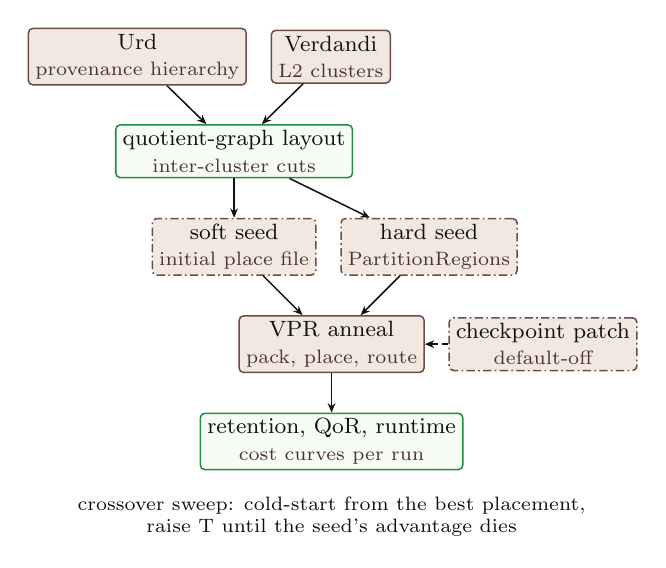
\begin{tikzpicture}[odin]
  % seed builders, side by side
  \node[box, neutral] (urd) {Urd\\\odinsub{provenance hierarchy}};
  \node[box, neutral, right=3mm of urd] (verd) {Verdandi\\\odinsub{L2 clusters}};
  \node[box, light, below=5mm of $(urd.south)!0.5!(verd.south)$] (quot) {quotient-graph layout\\\odinsub{inter-cluster cuts}};
  % injection, side by side
  \node[box, external, below=5mm of quot] (soft) {soft seed\\\odinsub{initial place file}};
  \node[box, external, right=3mm of soft] (hard) {hard seed\\\odinsub{PartitionRegions}};
  % VPR and the patch
  \node[box, neutral, below=5mm of $(soft.south)!0.5!(hard.south)$] (vpr) {VPR anneal\\\odinsub{pack, place, route}};
  \node[box, external, right=3mm of vpr] (ckpt) {checkpoint patch\\\odinsub{default-off}};
  % measurements
  \node[box, light, below=5mm of vpr] (met) {retention, QoR, runtime\\\odinsub{cost curves per run}};
  % flow
  \draw[flow] (urd) -- (quot);
  \draw[flow] (verd) -- (quot);
  \draw[flow] (quot) -- (soft);
  \draw[flow] (quot) -- (hard);
  \draw[flow] (soft) -- (vpr);
  \draw[flow] (hard) -- (vpr);
  \draw[flow, dash pattern=on 2.4pt off 1.4pt] (ckpt) -- (vpr);
  \draw[flow] (vpr) -- (met);
  % the sweep note
  \node[plain, below=3mm of met, font=\scriptsize\color{o3sub}, align=center]
    {crossover sweep: cold-start from the best placement,\\raise T until the seed's advantage dies};
\end{tikzpicture}
}
\caption{The seeding baseline. Seeds from provenance and recovered clusters, arranged by a quotient-graph layout, enter VPR softly (initial placement) or hard (constraints). The crossover sweep cold-starts from the best placement and raises the initial temperature until the seed's advantage dies or the sweep reaches its cap.}
\label{fig:norns}
\end{figure}

\subsection{Outside placers and run records}
\label{sec:i-tools}

\pp{Plain English.} To tell whether a finding belongs to VPR or to placement in general, we run a placer from outside the VTR tools, feed its result back into VPR, and let VPR route and time it, so every placer is judged by the same router and timer. Every run writes a record of what was run and where each parameter came from, so M\'{\i}mir can store it.

\pp{Technical.} A converter writes the outside placement (nextpnr HeAP or SA) in the flat-placement file format (\code{--read\_flat\_place}); a reread control reads VPR's own final placement back, and each ratio is within a family (analytic with analytic, annealing with annealing). Rule H0 fixes adders, multipliers, RAMs and pads at VPR's analytic positions, so the outside placers inherit part of VPR's solution and nextpnr has no timing model (both biases are in every table caption). Each run writes a \code{mimir-run.json} (\code{scripts/runrecord.py}).


\section{Methodology}
\label{sec:method}

\subsection{Setup}
\label{sec:setup}

Every experiment targets the VPR architecture \code{k6\_frac\_N10\_frac\_chain\_mem32K\_40nm} ($K=6$, ten BLEs per CLB, carry chains, 32\,Kb memories, multipliers). The netlist is the VTR-dialect BLIF that Odin~III's front end writes: \code{read\_verilog --nolatches --vtr-compat}, \code{proc}, \code{fsm}, \code{opt}, \code{flatten}, \code{opt -full}, \code{wreduce}, \code{hardmap}, \code{lower}, \code{abc --lut 6}, \code{stats}, \code{write\_blif --vtr --lut-k 6 --name-style provenance}. The seeding baseline runs on VPR \code{v8.0.0+18416} with one deterministic VPR seed per configuration. The packer experiments use VTR commit \code{3c9a4d23b2} (VTR~\cite{rose2012vtr}, VTR~9~\cite{elgammal2025vtr9}) with three VPR seeds per configuration unless the experiment says otherwise. The designs are: the 15 VTR~8.0 designs of Table~\ref{tab:benchmarks}; the generated yardstick designs (72, 105 and 84 designs, Section~\ref{sec:i-yardstick}); and for the option sweep 35 designs, the 20 MCNC circuits and the 15 designs of Table~\ref{tab:benchmarks}. Every number in the paper traces to a committed file, named in a comment at the number in the source, in the research log (\code{docs/paper/hypotheses.md}) or in \code{data/}. Raw run directories are not committed; their summaries are.

\subsection{Benchmarks}
\label{sec:benchmarks}

Table~\ref{tab:benchmarks} reports each design's construction and its post-technology-mapping size. The module count is the front end's, while the CLB count and the grid are VPR's own numbers for the packed netlist.

% BEGIN tab:benchmarks prose
The 15 designs span two orders of magnitude after technology mapping:
from 13 CLBs (ch\_intrinsics) to 1956 (stereovision2),
4843 CLBs in total. The mean is 322.9 CLBs and the median 125;
the mean sits well above the median because three stereovision designs carry most of the logic.
VPR auto-sizes a square grid to the packed netlist, with a mean side of 27.2 tiles
(median 20) and a mean of 1076.4 grid tiles (median
400). Grid size follows the largest resource demand, not the CLB count:
I/O-heavy and memory-heavy designs such as mkDelayWorker32B get a large die for few CLBs.
% END tab:benchmarks prose

\begin{table*}[t]
\caption{Benchmark construction and post-technology-mapping size. All fifteen
designs are from the VTR~8.0 benchmark set
(\code{vtr\_flow/benchmarks/verilog}). Modules is the front end's module
count, CLBs the \code{clb} blocks VPR packs, Memory and Mult the memory and
\code{mult\_36} blocks, and Grid the auto-sized device grid with its tile
count in parentheses. Sizes are read from each design's baseline run log and
kept in \code{data/benchmark-sizes.json}.}
\label{tab:benchmarks}
\centering
\footnotesize
\begin{tabular}{@{}l l r r r r c@{}}
\toprule
Design & Suite & Modules & CLBs & Memory & Mult & Grid (tiles) \\
\midrule
ch\_intrinsics & VTR 8.0 & 2 & 13 & 1 & 0 & $10\times$10 (100) \\
stereovision3 & VTR 8.0 & 1 & 15 & 0 & 0 & $7\times$7 (49) \\
diffeq2 & VTR 8.0 & 1 & 22 & 0 & 5 & $16\times$16 (256) \\
diffeq1 & VTR 8.0 & 1 & 37 & 0 & 5 & $16\times$16 (256) \\
mkPktMerge & VTR 8.0 & 7 & 21 & 15 & 0 & $28\times$28 (784) \\
raygentop & VTR 8.0 & 15 & 143 & 1 & 6 & $19\times$19 (361) \\
sha & VTR 8.0 & 1 & 142 & 0 & 0 & $17\times$17 (289) \\
boundtop & VTR 8.0 & 13 & 54 & 1 & 0 & $15\times$15 (225) \\
mkSMAdapter4B & VTR 8.0 & 8 & 125 & 5 & 0 & $20\times$20 (400) \\
or1200 & VTR 8.0 & 16 & 252 & 2 & 1 & $27\times$27 (729) \\
stereovision0 & VTR 8.0 & 25 & 707 & 0 & 0 & $33\times$33 (1089) \\
stereovision1 & VTR 8.0 & 16 & 788 & 0 & 43 & $40\times$40 (1600) \\
mkDelayWorker32B & VTR 8.0 & 16 & 74 & 43 & 0 & $50\times$50 (2500) \\
stereovision2 & VTR 8.0 & 24 & 1956 & 0 & 192 & $82\times$82 (6724) \\
blob\_merge & VTR 8.0 & 2 & 494 & 0 & 0 & $28\times$28 (784) \\
\bottomrule
\end{tabular}
\end{table*}


\subsection{Metrics}
\label{sec:metrics}

\pp{Area (low is better).} The LUT count of the Odin~III netlist, the number of logic CLBs after packing, the die grid VPR chooses, and the minimum routable channel width.

\pp{Speed (high is better): critical and near-critical.} The speed numbers are the critical-path delay (CPD) in nanoseconds and the near-critical statistics below. The routed wirelength (WL) is reported beside them as a proxy for wire delay and routing area; it is the primary metric of the packer experiments because their plans named it. A design is not fast only because its single slowest path is fast, since the next slowest path becomes the CPD once the first is sped up. We therefore also look at near-critical connections, those within 10\% of the CPD in the routed timing report. VPR defines the criticality of a connection from its slack, normalised by the CPD~\cite{luu2014thesis}; VPR~9 computes it relaxed per timing constraint~\cite{wainberg2015relaxed}. Only one near-critical statistic exists in this paper (the experiment of Section~\ref{sec:e-census}); worst slack per object is not yet measured (Section~\ref{sec:mimir}).

\pp{Power.} Power is not measured in any experiment of this paper. We make no claim about it, and we cite no relation of power to area.

\subsection{Hypotheses, experiments and verdicts}
\label{sec:verdicts}

Each experiment subsection of Section~\ref{sec:experiments} has the same four parts: the hypothesis in one sentence, the experiment (designs, arms, seeds), the result (numbers and the test), and the verdict. The verdict rule of each experiment is a numeric rule written in its plan file under \code{docs/plan/}; a rule is only changed by a dated entry that keeps the old text, and where a rule was changed the original verdict is the one reported. The four verdicts are:

\begin{itemize}
\item \textsc{useful}: supported under the experiment's rule, and not fragile.
\item \textsc{possibly good}: supported, but narrow or fragile (few designs, a clause added to the rule after the data, or a rule chosen after the data). It appears in the main text only with its fragility stated and is never the sole proof of an innovation.
\item \textsc{inconclusive}: the numbers do not decide. An experiment whose plan fixed no threshold in advance is \textsc{inconclusive} wherever the numbers do not decide; we never invent a threshold afterwards.
\item \textsc{dismissed}: not supported (failed). Dismissed ideas get one row in the research log (Appendix~\ref{sec:log}) and are argued here only where the paper's question needs the answer.
\end{itemize}

\subsection{Statistics}
\label{sec:stats}

Ratios are geometric means over designs of the variant over the reference; below 1 favours the variant for every metric of this paper. Where a rule uses a test, the sign test counts designs that improve, the Wilcoxon test is on the paired differences (on log ratios, one-sided where stated), the Holm adjustment corrects for the family of tests the plan names, and a bootstrap interval resamples the designs (10\,000 resamples, seed 20261026; 90\% or 95\% as stated). A permutation null shuffles labels. Designs are not independent draws from a population: an interval is over this set of designs.

\subsection{M\'{\i}mir as the instrument}
\label{sec:mimir}

M\'{\i}mir~III stores, for each placed object, its provenance, its coordinates and its timing, so each experiment above can be asked of the data as well as run. What it holds today for this work: \code{structure\_mapping} rows per design, structure, run and level, with the bounding box and spread of an HDL structure's CLBs and the structure's share of the critical path (\code{crit\_share}, only with a timing run); and the run fields \code{vpr.wirelength}, \code{vpr.chan\_width}, \code{vpr.cpd}, \code{vpr.worst\_slack}, \code{vpr.logic\_clbs} and the Norns fields (\code{norns.purity}, \code{norns.reproduction}, \code{norns.cut}, \code{norns.retention}, \code{norns.critical\_matched\_delay\_share}). What is missing: near-critical statistics per HDL object (only the single worst path gives a share, so the near-critical experiment of Section~\ref{sec:e-census} cannot be recomputed from M\'{\i}mir), worst slack per structure, and power, which has no field at all.


\section{Experiments}
\label{sec:experiments}

Each subsection states one hypothesis, the experiment, the result and the verdict. Numbers are from the files named in the comments of this source and in \code{docs/paper/hypotheses.md}. Tests that were not decided by the numbers are \textsc{inconclusive}; the full list, including every \textsc{dismissed} hypothesis, is in Appendix~\ref{sec:log}.

\subsection{Does the standard packer scatter the HDL's registers? (H8, H10a, H9a)}
\label{sec:e-scatter}

\pp{Hypothesis (H8).} The standard packer scatters the words of the HDL across CLBs: median word purity at most 0.80 and median split factor at least 1.5.
\pp{Experiment.} The 15 designs of Table~\ref{tab:benchmarks}, stock packing, word purity and split factor against a null that assigns the same atoms at random to CLBs of the same sizes (50 samples).
\pp{Result.} Median word purity 0.63 and median split factor 4.00; purity is above the random null on 15 of 15 designs. % data/analysis/r3-results.json H8: median_share 0.6255, median_split 4.0, above_null 15
\pp{Verdict.} \textsc{useful}.

\pp{Hypothesis (H10a).} Io-words give a word to LUTs that the front end's words left without one.
\pp{Experiment and result.} On the same 15 designs, the median gain in the share of LUTs that carry a label is 24.1\%, positive on 15 of 15 designs. % r3-results.json H10a median_gain 0.2411, positive 15
\pp{Verdict.} \textsc{useful}.

\pp{Hypothesis (H9a-word, H9a-wordio).} The Norns packer raises word purity with at most 5\% CLB growth.
\pp{Experiment.} 15 designs, three VPR seeds, source word and source word+io, $\beta$ from a grid chosen on the four smallest designs (which read only purity and CLB count).
\pp{Result.} Purity rises by 0.111 (word) and 0.104 (word+io), and by 0.120 and 0.124 without the four grid-choice designs; CLB count change 0.0\%; Holm-adjusted Wilcoxon $p<0.001$ for both. % hypotheses.md H9a-word, H9a-wordio; r3-results.json H9a
\pp{Verdict.} \textsc{useful}, as a mechanism check: purity is not an end metric. (Source module: purity gain 0.000, \textsc{inconclusive}.)

\subsection{How much room is there for a better packer? (H24, H27, H29--H31, H25/H19, H32, H20)}
\label{sec:e-room}

\pp{Hypotheses.} The yardstick is exact: synthesis keeps the construction and the \emph{known} arm reproduces the intended blocks (H24, H27, H29, H30, H31). The standard packer is worse than the known clustering by at least 5\% (H25, H19, H32). The Norns packer is still worse than the known clustering (H20).
\pp{Experiment.} The yardstick designs of Section~\ref{sec:i-yardstick}: 72 designs at the netlist level, 63 of the 72 at the HDL level that the label rule keeps, 105 alignment designs, arms stock, norns and known, three VPR seeds.
\pp{Result.} The known arm reproduces the blocks exactly (mean reproduction 1.000, 189 HDL runs and 216 netlist runs); the alignment manipulation works (Spearman 0.988 between designed alignment and measured purity; purity 0.100 at $a=0$ and 1.000 at $a=1$) and synthesis keeps the construction on 105 of 105 alignment designs. % r5-results.json repro_HDL, repro_NL; r6-results.json keep, repro, align
Stock over known, geometric mean: on the 72 netlist designs CLB 1.073, WL 1.220 [1.168, 1.275] (90\% interval), CPD 1.093; on the 63 HDL designs CLB 1.073, WL 1.219, CPD 1.082; on the mesh and tree alignment designs (14 cells) CLB 1.152, WL 1.489 [1.394, 1.591], CPD 1.181; Holm $p<0.001$ throughout. % hypotheses.md H25/H19, H32; r6-results.json room
The room depends on the topology: the stock WL ratio is 1.42 to 1.53 on mesh and tree and close to 1.0 on chain and random graphs, so the pooled 1.22 mixes designs with room and designs without. % r5-results.tex exploratory paragraph: NL stock mesh 1.423, tree 1.522, chain 1.004, rand 1.019; HDL stock mesh 1.444, tree 1.528, chain 1.027, rand 1.011
For the Norns packer on the 63 HDL designs, WL is still 1.099 [1.057, 1.147] of the known clustering (Holm $p=0.003$); CLB (1.031) and CPD (1.032) are \textsc{inconclusive}. % r5-results.tex H20
These HDL designs include the \code{dp} designs whose word file is the leak (Section~\ref{sec:e-leak}), so H20 describes the packer with the hint; it does not say how much room remains with realistic words.
\pp{Verdict.} \textsc{useful} (validity, H25/H19, H32, and H20 for WL). Limits of the yardstick are in Section~\ref{sec:limits}.

\subsection{How far is the packer from a known optimum on real designs? (H38, round 9)}
\label{sec:e-real}

\pp{Hypothesis (H38).} On real designs made into known-optimum yardsticks (Section~\ref{sec:i-yardstick-real}), the standard packer is worse than the known clustering by at least 5\% in CLBs, wire or delay. The rule is that of the synthetic yardstick: \emph{room} if the geometric mean of stock over known is at least 1.05 and the 90\% bootstrap interval of the mean log ratio excludes 0; \emph{no room} if the mean is at most 1.02 or the interval lies inside [0.98, 1.02]; otherwise inconclusive. With fewer than 12 designs no pooled claim is made.
\pp{Experiment (pilot).} Three designs (ch\_intrinsics, diffeq1, mkPktMerge: 12 to 42 clusters, with memory slices and multipliers), each built with the own and the foreign clustering, three shuffles, three VPR seeds, arms stock and known (108 runs), plus 18 stock runs on the unshuffled \emph{ordered} files. Flow flags and architecture as the synthetic yardstick (VTR commit \code{3c9a4d23b2}~\cite{rose2012vtr,murray2020vtr8}). Table~\ref{tab:r9pilot}.
\pp{Result.} The known arm needs 1.02 to 1.11 times the exact CLB count $K$ and reproduces 40\% to 80\% of the clusters; the standard packer needs 1.06 to 1.19 times $K$. The room is small on two designs and larger on the smallest: stock over known is 1.13 in CLBs and 1.09 to 1.14 in wire on ch\_intrinsics, between 1.007 and 1.075 on the other two, and the delay ratio is between 0.98 and 1.07 (room only on ch\_intrinsics with the own clustering). No design shows the 1.49 of the synthetic meshes and trees. The ordered control has stock purity within 0.06 of the shuffled arm on all six builds, higher by at most 0.04 and lower once (0.80 against 0.85 on ch\_intrinsics own), so file order gives the packer no visible advantage. The wire gap is larger on the foreign build than on the own build for all three designs (by 0.05, 0.03 and 0.01), which is the direction a small advantage to VPR on its own clustering would take, but three designs cannot separate self-bias from design. % data/r9/pilot-summary.json
\pp{Verdict.} \textsc{inconclusive} (3 designs; the rule needs 12). The row is the pilot and not the answer. The comparison with the synthetic yardstick is a pointer only: on these three designs the artificial regularity did not hide a larger gap.

\begin{table}[t]
\caption{H38 pilot: stock over known (geometric mean over 3 shuffles $\times$ 3 seeds) and CLB counts against the exact bound $K$. Status by the rule of the text: R room, N no room, I inconclusive. Source: \code{data/r9/pilot-summary.json}.}
\label{tab:r9pilot}
\centering
\footnotesize\setlength{\tabcolsep}{3pt}
\begin{tabular}{@{}llrrrrrr@{}}
\toprule
Design & C & $K$ & stock/$K$ & known/$K$ & CLB & WL & CPD \\
\midrule
ch\_intrinsics & own & 12 & 1.19 & 1.06 & 1.13\,R & 1.09\,R & 1.06\,R \\
ch\_intrinsics & foreign & 12 & 1.19 & 1.06 & 1.13\,R & 1.14\,R & 0.98\,N \\
diffeq1 & own & 42 & 1.14 & 1.11 & 1.02\,I & 1.01\,N & 1.02\,N \\
diffeq1 & foreign & 41 & 1.11 & 1.10 & 1.02\,N & 1.03\,I & 1.00\,N \\
mkPktMerge & own & 22 & 1.06 & 1.03 & 1.03\,I & 1.01\,N & 0.99\,N \\
mkPktMerge & foreign & 22 & 1.09 & 1.02 & 1.07\,R & 1.02\,N & 1.02\,N \\
\bottomrule
\end{tabular}
\end{table}

\pp{Full set.} \todo{round 9 full: 15 Verilog designs and 20 MCNC designs, own and foreign, table to be filled after the full-set pull request merges; the verdict of H38 is then re-stated on that table}

\subsection{Does the packer pay when the words equal the blocks? The leak (H33, H36, H35, H34, H22, H23)}
\label{sec:e-leak}

\pp{Hypotheses.} (H33) With words equal to the blocks the Norns packer beats stock. (H36) Its gain grows with the measured alignment. (H35) It makes WL worse by at least 2\% when the words do not match the blocks. (H34) It beats stock at each alignment below 1. (H22) On the 63 HDL designs of the first yardstick round it beats stock.
\pp{Experiment.} The 105 alignment designs; 14 designs per alignment level (mesh and tree, seven sizes); Norns over stock, three seeds.
\pp{Result.} At $a=1$ (words equal blocks) Norns/stock is CLB 0.870, WL 0.669 [0.627, 0.713], CPD 0.841 (H33). % r6-results.json leak_a1
Below 1 it is worse: WL 2.034, 2.038, 1.731 and 1.218 of stock at $a=0$, 0.25, 0.5 and 0.75 (Holm $p<0.001$ for harm at every level; H35), so no leak-free level shows a gain (H34). % r6-results.json hurt
The slope of the WL ratio on the measured alignment is negative in 14 of 14 cells (median $-1.317$; $-0.786$ on the leak-free levels only; Holm $p<0.001$; H36). % r6-results.json dose, dose_leakfree_variant
The first yardstick round had reported WL 0.902 [0.866, 0.936] of stock on 63 HDL designs (H22). % r5-results.json close_HDL
That gain sits only in the \code{dp} designs, whose word file equals the block partition (purity 0.9998), and is zero in the 27 \code{ctl} designs, where the Norns \code{.net} equals the stock \code{.net} on 27 of 27; the purity gain is zero when the HDL has no vector (median difference 0.000; H23). % r5-results.json leak_HDL, h23; round8-h22.md
\pp{Verdicts.} H33, H36, H35: \textsc{useful}; H33 is an upper bound, because the words equal the blocks, and H35 is a finding about harm. H34: \textsc{dismissed}. H23: \textsc{dismissed} as stated. H22: \textsc{dismissed}: its gain is withdrawn as a result. It was an oracle leak and is reported here only as a finding about method.

\subsection{With realistic words, does the packer reduce wirelength? (H22$'$, H37)}
\label{sec:e-h22p}

\pp{Hypothesis (H22$'$).} With bus words that do not mirror the CLB partition, the Norns packer reduces WL against stock.
\pp{Experiment.} 84 generated designs (Section~\ref{sec:i-leak}): mesh and tree, four word widths $w$, seven sizes (14 designs per width), and chain controls (seven per width); arms stock, norns ($\beta=4$) and known; three seeds; 798 runs, all completed. Two controls ran first: at $\beta=0$ the Norns \code{.net} must equal stock's (28 of 28 chain designs byte-identical), and at alignment 1 on chain Norns/stock must be about 1.00 (1.003 [0.993, 1.013]; both passed). The hypothesis is supported if the WL geometric mean is at most 0.99 with Holm $p<0.05$, and not supported if it is at least 1.00 or its 90\% interval lies inside [0.98, 1.02].
\pp{Result.} Table~\ref{tab:h22p}. The packer raises WL by 65\% to 150\% at every width, and CPD by 33\% to 41\%; Holm-adjusted $p=1.0$ at every width. It reduces the CLB count by 2.7\% and 5.4\% at $w=16$ and 32 (Holm $p=0.0015$, $0.0010$) and raises it at $w=4$ and 8; a CLB result never changed the WL verdict. The chain control fails at every width, so no mesh or tree figure may be read as a gain. The known grouping reaches 0.672 of stock WL on mesh and tree at every width: the headroom is real, and realistic words do not reach it.

\begin{table}[t]
\caption{H22$'$: Norns over stock, mesh and tree pooled (14 designs per width), geometric mean with the 90\% bootstrap interval; and the chain control (7 designs). Below 1 favours Norns. Source: \code{data/analysis/r8-results.json}.}
\label{tab:h22p}
\centering
\footnotesize
\begin{tabular}{@{}rcccr@{}}
\toprule
$w$ & WL [90\%] & CPD & CLB & chain WL \\
\midrule
4 & 1.652 [1.525, 1.809] & 1.329 & 1.033 & 3.575 \\
8 & 2.011 [1.824, 2.237] & 1.371 & 1.012 & 5.604 \\
16 & 2.349 [2.125, 2.609] & 1.380 & 0.973 & 7.969 \\
32 & 2.505 [2.247, 2.802] & 1.407 & 0.946 & 9.497 \\
\bottomrule
\end{tabular}
\end{table}

\pp{The chain control, per alignment level (H37).} The first control, pooled over alignment levels, gave Norns/stock 4.15 on 35 chain designs, and was read as a failed control. The pooled number averages over levels. Per level (chain, WL Norns/stock, $n=7$ each): $a=0$ 8.71, $a=0.25$ 8.37, $a=0.5$ 6.19, $a=0.75$ 2.72 and $a=1$ 1.003. % r8-results.json h37_per_level
At $a=1$ the packer leaves chain unchanged. The harm grows as word purity falls (median purity 0.10, 0.26, 0.51, 0.75, 1.00). The pooled control was ill-posed: chain has no headroom, not no effect, and a packer that follows misaligned words is expected to do harm there. The H22$'$ word files have median purity 0.26 at $w=4$ down to 0.07 at $w=32$, and the harm grows with $w$ in the same way. The mechanism is consistent with the packer pulling flip-flops of different blocks into one CLB because they share a word; it was not measured directly (no per-CLB mixing was counted, and width, purity and words per block change together).
\pp{Verdicts.} H22$'$: \textsc{dismissed} (not confirmed at any of the four widths). H37: \textsc{dismissed}, as a control that was ill-posed; the per-level figures above replace it. Not tried: a smaller $\beta$, words that only partly agree with the blocks, and real HDL words (Section~\ref{sec:future}).

\subsection{Are near-critical connections kept inside CLBs? (H17c)}
\label{sec:e-census}

\pp{Measurement (H17a, not a hypothesis).} Over 15 designs with stock packing, the median share of CLB pairs that are series-critical is 4.0\%, shared-input or orthogonal 32.0\%, and series-noncritical or filler 64.4\%. % r4-results.json n17 H17a median_SC 0.0403, median_SI_OR 0.3200, median_SN_FL 0.6443
\pp{Hypothesis (H17c).} Near-critical edges (within 10\% of the CPD) cross CLB boundaries less often than edges in general under the standard packer.
\pp{Experiment.} The 9 designs with at least 20 near-critical hops, routed timing reports.
\pp{Result.} Median rate ratio 0.652 (near-critical over all edges), one-sided Wilcoxon $p=0.027$. % r4-results.json n17 H17c
\pp{Verdict.} \textsc{possibly good}. It passes the rule as written, on 9 designs; it would fail a minimum of 12 designs that was not part of the rule text, and the design set is small. It is the only near-critical statistic in this paper. The Norns packer does not change the series-critical share (median change $-0.003$; H17b, \textsc{dismissed}).

\subsection{What do VPR's options do to area and speed? (E10)}
\label{sec:e10}

\pp{Hypotheses.} Nine one-factor hypotheses around the base flow (the annealing placer, the default ABC script, $K=6$, the \code{k6\_frac} architecture): two other ABC scripts; $K=4$ (which also removes the hard blocks); the EArch architecture; unrelated clustering forced on and forced off; VPR's analytic placer; nextpnr HeAP and SA through the flat-placement file.
\pp{Experiment.} 35 designs (20 MCNC, 15 from Table~\ref{tab:benchmarks}), three seeds, one factor against the base. The comparisons were fixed, no thresholds were. We call a measure supported only if its 95\% design-bootstrap interval excludes 1.000 \emph{and} its Holm-adjusted $p$ (36 tests) is below 0.05.
\pp{Result.} Table~\ref{tab:e10}. The area and speed measures move in different directions. The area-oriented ABC script lowers the LUT count by 3.0\% and raises the CPD by 14.1\%. The EArch architecture lowers the CLB count by 14.5\% and raises WL by 16.0\%. Unrelated clustering lowers the CLB count by 7.6\% with no supported change in CPD or WL. The analytic and nextpnr placers lower WL by 4.3\% to 5.0\% and raise the CLB count by 3.1\% to 4.0\%, with the CPD not decided. Forcing unrelated clustering off changes nothing: all four ratios are exactly 1.000. % data/e10/ratios.csv, docs/plan/e10-hypotheses.md
\pp{Verdict.} Eight of the nine are \textsc{possibly good}: each has at least one measure that survives the adjustment, but the verdict rule is post hoc, the design set is not a sample of a population, $K=4$ is confounded with the removal of the hard blocks, and the external placers inherit VPR's hard blocks and pads (rule H0) and nextpnr has no timing model. The last (forced off) is \textsc{dismissed} as a no-op. Measures whose interval excludes 1.000 but whose Holm $p$ is not below 0.05 (for example the LUT count and CPD of ABC script 1) are \textsc{inconclusive}.

\begin{table*}[t]
\caption{E10: ratio of each level to the base flow (annealing placer), geometric mean over designs; * marks a measure whose 95\% interval excludes 1.000 and whose Holm $p<0.05$ (supported); = marks a byte-identical ratio. Below 1 is better. $n=35$ except $K=4$ (33--34) and the nextpnr arms (30 on CLBs, CPD and WL). Source: \code{data/e10/ratios.csv}.}
\label{tab:e10}
\centering
\footnotesize
\begin{tabular}{@{}lcccc@{}}
\toprule
Level & LUTs & CLBs & CPD & WL \\
\midrule
ABC script 1 (rewriting) & 1.103 & 1.114* & 1.027 & 1.113* \\
ABC script 2 (area-oriented) & 0.970* & 0.970 & 1.141* & 0.985 \\
$K=4$ architecture & 1.974* & 5.320* & 1.488* & 1.288 \\
EArch architecture & 1.000= & 0.855* & 1.004 & 1.160* \\
unrelated clustering on & 1.000= & 0.924* & 0.996 & 1.001 \\
unrelated clustering off & 1.000= & 1.000= & 1.000= & 1.000= \\
VPR analytic placer & 1.000= & 1.040* & 1.005 & 0.957* \\
nextpnr HeAP & 1.000= & 1.032* & 1.011 & 0.950* \\
nextpnr SA & 1.000= & 1.031* & 1.018 & 0.955* \\
\bottomrule
\end{tabular}
\end{table*}

\subsection{Does starting placement from the designer's grouping help? (R1, H4)}
\label{sec:e-seed}

\pp{Hypothesis (R1a).} A seeded start gives better placement than VPR's own analytic start when the anneal begins at VPR's own temperature.
\pp{Experiment.} The 15 designs of Table~\ref{tab:benchmarks}; seven seed families (Urd and six recovered, Section~\ref{sec:i-seed}) in a soft arm with the full intra-cluster order or shuffled; one VPR seed.
\pp{Result.} Table~\ref{tab:qor}. Soft seeds stay within a few percent of the baseline: geomean WL 0.997 to 1.029 across families, 1.009 pooled, with the channel width lower (0.947 to 0.994) and the placement runtime 1.07 to 1.09 times longer. % hypotheses.md R1a; norns.tex tab:qor (earlier version); EXP:25-72
Hard floorplan regions are worse (geomean WL 1.088 over 104 runs; R1c, \textsc{dismissed}). The crossover sweep finds a median crossover of $16\times$ (range $4\times$ to $256\times$), and at twice the crossover the seeds win only 57 of 105 head-to-heads against an unseeded run at the same temperature (R1e). The best placement over all seeds, $P^*$, is the best of about 20 placements and no control restarts the anneal with equal effort, so part of the crossover may be selection. A random start is as good as any seed: with Urd the WL ratio is 0.997 from a random start, 1.020 from permuted clusters and 1.029 from the quotient layout (H4, \textsc{dismissed}).
\pp{Verdict.} R1a and R1e: \textsc{inconclusive}. The honest answer is that seeding at VPR's own temperature has no measured gain on 15 designs and one VPR seed, and this is why the paper moved to the packer.

\begin{table}[t]
\caption{Seeding baseline: geomean quality ratios against the unseeded baseline, soft arm (15 designs, one VPR seed); the inter-cluster-only row shuffles the order inside each cluster and pools all seven families, and the $k$-means row pools $k$, $2k$ and $4k$. Below 1.0 is better. Source: \code{docs/plan/EXPERIMENT.md} (round one).}
\label{tab:qor}
\centering
\footnotesize
\begin{tabular}{@{}lrrrr@{}}
\toprule
Seed & Wirelength & Delay & Chan. width & Runtime \\
\midrule
Urd (hierarchy) & 1.029 & 1.004 & 0.958 & 1.068 \\
Louvain & 1.008 & 0.982 & 0.980 & 1.091 \\
Spectral & 1.006 & 0.993 & 0.968 & 1.098 \\
Affinity propagation & 1.002 & 1.003 & 0.982 & 1.086 \\
$k$-means ($k$, $2k$, $4k$) & 1.006 & 0.985 & 0.975 & 1.088 \\
Inter-cluster only & 1.015 & 0.981 & 0.987 & 1.102 \\
\bottomrule
\end{tabular}
\end{table}

\subsection{Is the hierarchy physical on the chip? (H11)}
\label{sec:e-hier}

\pp{Hypothesis.} CLB pairs of the same word, or of the same module, sit closer on the annealed placement than their net connectivity alone predicts.
\pp{Experiment.} Stock packing, analytic start, three VPR seeds; the stratified mean distance difference of related over unrelated pairs as a fraction of the unrelated distance (negative is closer), against a permutation null.
\pp{Result.} Same-word median $-0.176$ ($p=0.017$; 9 of 12 designs sign-consistent, 12 required); same-module median $-0.188$ ($p<0.001$; 10 of 11, 12 required). % hypotheses.md H11; r3-results.tex
\pp{Verdict.} \textsc{inconclusive}: the pairs are closer, but the count of designs that the rule requires cannot be reached on the 11 or 12 designs that qualify.

\subsection{How much would hindsight gain, and do other placers agree? (R7a, R8a, R8b)}
\label{sec:e-hind}

\pp{Hypothesis (R7a).} Re-clustering according to where the best stock placement put atoms lowers WL$\times$CPD on held-out seeds.
\pp{Experiment.} 1660 VPR runs; the arm is chosen on seeds 1--5 and measured on seeds 6--10; 15 designs, 8 with a chosen arm.
\pp{Result.} Held-out median WL gap 0.987, CPD gap 0.994, CLB gap 1.026; the objective interval lies above 1 on 1 of 8 designs (7 borderline); 7 of the 15 designs are imputed as 1. % r7-abstract.tex; r7-results.tex
\pp{Verdict.} \textsc{inconclusive}: little evidence of room that a better clustering with hindsight would capture.

\pp{Hypotheses (R8a, R8b).} nextpnr HeAP lands where VPR's analytic placer does, and nextpnr SA places with equal or less wirelength than VPR's annealer.
\pp{Experiment.} 13 eligible designs, seeds 4--6 held out, ratios within a family against the reread control, design bootstrap.
\pp{Result.} HeAP over reread: WL 1.001 [0.984, 1.019], CPD 1.027 [1.009, 1.046], WL$\times$CPD 1.028 [0.996, 1.061]. SA over reread: WL 0.947 [0.919, 0.975], CPD 1.003 [0.973, 1.039], WL$\times$CPD 0.952 [0.909, 1.003]. % r8-results.tex tab:r8family; placers.md Section 10.9 as corrected by 10.10
\pp{Verdict.} Both \textsc{inconclusive}: the WL$\times$CPD intervals include 1; rule H0 means the outside placers inherit VPR's hard blocks and pads; neither outside placer is timing-driven.


\section{Summary of What Was Tried}
\label{sec:summary}

Table~\ref{tab:tried} lists every change to packing or placement that this work tried in the hope of a deployable gain, and the one oracle that bounds what such a change could reach. It is read as a CAD paper is read. Each cell is the geometric-mean percent win over the stock flow (positive is better; a ratio of 1.007 stock over arm is a 0.7\% win) and, in brackets, the wins, losses and ties over designs (a tie is within 0.5\%). The columns are in the order speed (post-route critical-path delay, CPD), wirelength (WL), area (CLBs used). The last column is the strict register verdict (a positive geomean whose interval touches 1 is \textsc{inconclusive}, not \textsc{dismissed}). Every number is a row of the register (\texttt{docs/paper/hypotheses.md}).

\begin{table*}[t]
\centering
\caption{Every packing or placement change tried, with its CAD headline (geomean percent win; wins/losses/ties over designs in brackets; ``n/t'' = not tabulated in the register, the ratio is given instead). Real designs are the 35 of E10 (15 VTR Verilog, 20 MCNC) unless the row says 33 (round-9 known-optimum designs).}
\label{tab:tried}
\footnotesize
\setlength{\tabcolsep}{3pt}
\begin{tabular}{@{}p{3.9cm}p{2.9cm}p{2.9cm}p{2.9cm}p{3.6cm}@{}}
\toprule
Change (register ID) & Speed (CPD) & Wirelength & Area (CLBs) & Verdict \\
\midrule
Seeding the anneal from the designer's grouping (R1a, 15 designs) & ratio 0.970 to 1.004 (n/t) & ratio 0.997 to 1.029, pooled 1.009 (n/t) & channel width ratio 0.947 to 0.994 (n/t) & \textsc{inconclusive} (no gain in WL; no test) \\
HDL-aware packer, realistic registers (H22$'$, 56 mesh/tree designs) & 33 to 41 percent worse (ratio 1.33 to 1.41, n/t) & 65 to 150 percent worse (ratio 1.652 to 2.505, n/t) & ratio 0.946 to 1.033 (n/t) & \textsc{dismissed} at every width \\
Refresh criticality, every cluster (H-refresh k=1) & $-0.5$ (n/t; ratio 1.005 [0.990, 1.021]) & $-0.3$ (n/t) & $-0.2$ (n/t) & \textsc{inconclusive} \\
Refresh criticality, every 8th cluster (k=8) & $-0.7$ (n/t; ratio 1.007) & $-0.4$ (n/t) & $-0.5$ (n/t) & \textsc{dismissed} \\
Seed rule from the answer key (HS0, 33 designs) & $-0.8$ (n/t) & $+0.7$ (n/t) & $+0.7$ [18/13/2] & \textsc{inconclusive} \\
2-hop gain term, $w=0.1$ (H-2hop) & $+0.7$ [17/14/4] & $-0.2$ [15/16/4] & $-0.6$ [9/14/12] & \textsc{inconclusive} \\
2-hop gain term, $w=0.25$ & $-1.9$ [15/17/3] & $-1.0$ [13/17/5] & $+0.1$ [12/11/12] & \textsc{dismissed} \\
Spare room $s=2$, E10 flow (H-spare-2) & $-1.4$ [12/21/2] & $-2.2$ [7/22/6] & $-10.8$ [5/27/3] & \textsc{inconclusive} \\
Spare room $s=2$, fixed width & $-1.6$ [10/21/3] & $-2.3$ [6/27/1] & $-10.7$ [5/26/3] & \textsc{dismissed} \\
Spare room $s=4$, E10 flow & $-1.5$ [10/23/2] & $-3.1$ [6/26/3] & $-16.5$ [4/30/1] & \textsc{dismissed} \\
Spare room $s=4$, fixed width & $-2.1$ [10/20/3] & $-2.6$ [6/23/4] & $-16.8$ [4/28/1] & \textsc{dismissed} \\
Duplicate critical LUTs after placement, fixed width (H-dup-W) & $-0.5$ [11/20/4] & $-0.1$ [10/17/8] & $-1.1$ [0/20/15] & \textsc{dismissed} \\
Duplication after $s=2$ packing, fixed width (H-dup-spare-W) & $-0.4$ [12/20/2] & $-2.5$ [5/26/3] & $-10.3$ [4/27/3] & \textsc{dismissed} \\
\midrule
\multicolumn{5}{@{}l}{\textit{Bounds, not deployable (they use the answer key)}} \\
True seed oracle (Q-N1b, 33 designs) & $-0.7$ [13/20/0] & $+2.8$ [25/8/0] & $+1.2$ [23/6/4] & \textsc{possibly good} in WL and area, \textsc{inconclusive} in speed; strong form \textsc{dismissed} \\
HDL-aware packer, registers equal blocks (H33, 14 designs) & ratio 0.841 (n/t) & ratio 0.669 (n/t) & ratio 0.870 (n/t) & \textsc{useful} as an upper bound; a leak \\
\bottomrule
\end{tabular}
\end{table*}

Three things stand out. First, no deployable change wins on speed: the best geomean delay win is 0.7\% (H-2hop at $w=0.1$), with 17 wins against 14 losses, inside the noise. Second, the changes that move area or wire move them the wrong way (spare room raises CLBs by 11 to 17\%). Third, the two selections that looked like speed gains were selections: the duplication result of $+1.9$ and $+2.8$\% (setting a) is the best of up to five routed rounds scored on the number it is chosen on, and the same netlists routed afresh are 0.5 and 0.4\% slower; the original HDL-aware gain (WL 0.902 of stock) was a leak. Table~\ref{tab:tried} does not list the sweep of VPR options (E10), which changes tool settings and not the packer; its eight area and speed effects are in Section~\ref{sec:e10}.

What was measured, not tried, is the other half of the picture (all in the register). On 33 real designs made into known-optimum yardsticks (H38) the stock packer uses 1.103 times the proven lower bound on CLBs (corrected bound; 1.108 [1.080, 1.149] before the correction), and 1.265 times the wire and 1.026 times the delay of the known clustering over the 33 designs (delay \textsc{inconclusive}). Its decision log (Q-N2) puts 60\% of the CLB gap in picks of an atom of another known cluster while the right atom was queued, with a strictly lower gain in 99.8\% of them; 11\% comes from clusters closed with free slots. No C-free feature ranks the right atom well once the construction's dummy cells are deleted (Q-N3: AUC 0.687 [0.662, 0.711] with them, 0.612 without), and a seed oracle rebuilds only 25.5\% of known clusters exactly and closes 11\% of the log gap (Q-N1b). The measured room is real in CLBs and wire; what a rule that sees only the circuit can reach of it is, on these experiments, within noise.


\section{Discussion and Limits}
\label{sec:discussion}

\pp{What the experiments say.} The designer's grouping is physically real on the chip (H11, \textsc{inconclusive} by the letter of the rule), and the standard packer loses it (H8). A packer that is told the grouping can keep it (H9a), and when the grouping is exactly the right clustering it uses far less wire (H33: 0.669 of stock). But the same packer, handed registers that cut across the blocks, makes wirelength worse by 65\% to 150\% (H22$'$), and the harm falls as the registers line up with the blocks (H37 per level, H35, H36). The known-optimum yardstick shows the room is real: the known grouping reaches 0.672 of stock wirelength on meshes and trees at every register width (H22$'$) and the standard packer is 1.49 times it (H32). The honest reading is that in these experiments the gain appeared only when the hint was perfect: no alignment below 1 showed one, and our packer at $\beta=4$ does not degrade gracefully.

\pp{The leak as a method lesson.} The original gain (0.902 of stock) was real arithmetic on a flawed input: the word file was the answer. The yardstick caught it because it lets us dial the alignment, and because we reran with words that cut across blocks. A packer or placer claim on constructed benchmarks should always be accompanied by a control in which the hint is useless and one in which it is perfect.

\pp{Multi-metric view.} Area and speed move in different directions: the area-oriented ABC script lowers the LUT count and raises the CPD (E10); the outside placers lower WL and raise the CLB count; the packer lowers CLBs at wide words and raises WL and CPD (H22$'$). A result on one metric is not a result on the problem. Speed is judged here by the CPD and, only once, by the near-critical statistic (H17c). Power is not measured.

\subsection{Limits}
\label{sec:limits}

\begin{itemize}
\item \textbf{Few, small designs.} The real designs are 15 small VTR circuits; the seeding baseline used one VPR seed per configuration. Intervals are over this set of designs and not over a population.
\item \textbf{Constructed designs.} The yardstick designs and the H22$'$ words are generated. The word layout of H22$'$ is a random permutation, the extreme of misalignment; real buses may lie between that and the leak, and are untested (Section~\ref{sec:future}).
\item \textbf{The yardstick is a clustering optimum.} It is exact for CLB count and not a proven placement optimum. Synthesis keeps the construction in only 32 of 72 HDL designs under the original label rule (63 under an amended rule), and the netlist-level zero-violation check passes on 37 of 72 (H18, H28, \textsc{dismissed} by their literal rules); the analysis uses the 63 designs the amended rule keeps, and the netlist-level variants chosen after the data are labelled.
\item \textbf{An erratum.} The affinity files of the first packer experiments left out every adder (carry-chain) atom; H9 and H10 describe a packer that did not see carry chains. The later experiments (H22$'$ and the alignment designs) use corrected files.
\item \textbf{Near-critical evidence is thin.} H17c has 9 designs and \textsc{possibly good}; M\'{\i}mir cannot yet recompute it (Section~\ref{sec:mimir}).
\item \textbf{Outside placers.} Rule H0 and the lack of a timing model in nextpnr bias every comparison against VPR's own placers.
\item \textbf{E10.} The verdict rule is post hoc, $K=4$ is confounded with the removal of the hard blocks, and some arms exclude designs where a run failed.
\item \textbf{Power} is not measured.
\end{itemize}

\section{Future Work: Untested Hypotheses}
\label{sec:future}

Five ideas have no result yet. Each is stated with the one experiment it needs.

\pp{U1: a smaller $\beta$.} A smaller affinity weight may keep words without the harm seen at $\beta=4$ on misaligned words. Experiment: re-run H22$'$ on the same 84 designs over a ladder of $\beta$ below 4 with the same rule.
\pp{U2: partly aligned words.} Words that agree only partly with the blocks, may give a gain or a smaller harm. Experiment: re-run H22$'$ with words drawn at a controlled partial alignment on the realistic bus layout.
\pp{U3: real HDL words.} Real HDL words may behave like the constructions. Experiment: run stock and norns on the 15 VTR designs with the word files as written and test WL with the H22$'$ rule.
\pp{U4: crossover versus selection.} The crossover of the seeding baseline may reflect the seed and not selection of the best of about 20 placements. Experiment: an equal-effort control that restarts the anneal from the best of $N$ unseeded runs.
\pp{U5: packing for near-critical paths.} A packer that weights near-critical connections may improve the near-critical statistics. Experiment: per-object near-critical statistics in M\'{\i}mir (the top-$k$ or within-10\% paths) and a packer arm that uses them.

\section{Conclusion}
\label{sec:conclusion}

Keeping the designer's grouping through packing is a sound idea and a measurable one: the standard packer scatters the source's registers, a packer with an affinity bonus keeps them, and a yardstick with a known best grouping shows real room. But we could not show a gain from it. The one gain we measured came from a leak, and with realistic registers the packer used more wire at every setting we ran. Starting placement from the designer's grouping gave no measured benefit either. What the work does deliver is the instrument: the yardstick with an adjustable hint, the controls that expose a leak, and the run records that M\'{\i}mir stores so that area, speed and, once it is measured, power can be traced back to the HDL that caused them.


\appendices
\section{Research Log}
\label{sec:log}

Every hypothesis of the work, one row each, including the \textsc{dismissed} ones. The full register, with the experiment, metrics, test and source file of each row, is \code{docs/paper/hypotheses.md}. The counts are 14 \textsc{useful}, 9 \textsc{possibly good}, 21 \textsc{inconclusive}, 17 \textsc{dismissed} and one measurement (H17a), 62 rows in all. A row that groups related hypotheses (for example H34a--d) counts once.

% Generated by a one-off script from docs/paper/hypotheses.md rows; edit by hand if the register changes.
\begin{table*}[t]
\caption{Research log (1 of 3): every hypothesis, one row each. Verdicts as defined in Section~\ref{sec:verdicts}. Numbers are from the files named in \code{docs/paper/hypotheses.md}.}
\label{tab:log1}
\centering\footnotesize\setlength{\tabcolsep}{3pt}
\begin{tabular}{@{}p{0.7in}p{2.4in}p{2.75in}p{0.85in}@{}}
\toprule
ID & Hypothesis & Result & Verdict \\
\midrule
\multicolumn{4}{@{}l}{\textit{Rounds 1 and 2 (seeding)}} \\
R1a & Seeded start beats VPR's start at its own temperature & WL 0.997 to 1.029 across 7 families; pooled 1.009; one seed & \textsc{inconclusive} \\
R1b & Provenance (Urd) and recovered clusters seed differently well & Urd soft 1.029 (worst), Urd hard 1.062 (best hard); order flips & \textsc{inconclusive} \\
R1c & Hard floorplan regions help & Hard WL 1.088 over 104 runs, worse than soft & \textsc{dismissed} \\
R1d & Intra-cluster order matters beyond the coarse layout & WL 1.009 (full) vs 1.015 (inter), mixed signs & \textsc{inconclusive} \\
R1e & Cluster-derived start keeps winning when the anneal starts hotter & Median crossover $16\times$; seeds win 57 of 105 at $2\times$ & \textsc{inconclusive} \\
R1f & Checkpointing extends the useful temperature range & Same crossover on 14 of 15 designs & \textsc{dismissed} \\
H7a & Word seeds beat module seeds & WL 0.986, better on 10 of 15; sign test $p=0.302$ & \textsc{inconclusive} \\
H7b & Bit-sliced layout beats plain word clusters & WL 0.982 ($p=0.791$); channel width 1.033 & \textsc{inconclusive} \\
H7c & Hierarchy plus bit-slices has the lowest WL of 11 families & Ranks 8 of 11 (1.014) & \textsc{dismissed} \\
H7d & Seeding only the word CLBs beats the full word seed & WL 0.980, better on 9 of 15; $p=0.607$ & \textsc{inconclusive} \\
H4 & Order random > permuted > quotient $\geq$ analytic start & Urd 0.997, 1.020, 1.029: a random start is as good as any seed & \textsc{dismissed} \\
H1 & VPR's placement is module- and word-coherent & Above null+2sd on 8/11 (module) and 9/15 (word) designs; needs 2/3 & \textsc{inconclusive} \\
H2 & Seed gain correlates with design structure & 0 of 9 correlations positive at $p<0.05$ & \textsc{inconclusive} \\
\midrule
\multicolumn{4}{@{}l}{\textit{Round 3 (packing dilutes structure; the Norns packer)}} \\
H8 & Stock packing scatters HDL words & Word purity 0.63, split factor 4.00 & \textsc{useful} \\
H9a-module & Affinity packing raises module purity & Purity +0.000, CLB $-1.6$\% & \textsc{inconclusive} \\
H9a-word & Affinity packing raises word purity, CLB growth $\leq5$\% & Purity +0.111, CLB 0.0\%, $p<0.001$ (mechanism check) & \textsc{useful} \\
H9a-wordio & Same with word+io source & Purity +0.104, CLB 0.0\% (mechanism check) & \textsc{useful} \\
H9b & Affinity packing alone changes WL & WL 1.051 / 1.032 / 1.030 (module / word / word+io), $p$ 0.09 to 0.19 & \textsc{inconclusive} \\
H9c & Affinity packing plus word seed beats stock plus word seed & WL 1.064 / 1.039 / 1.039, better on 2 to 5 of 15 & \textsc{dismissed} \\
H10a & Io-words label LUTs that had no word & Median coverage gain 24.1\%, 15 of 15 designs & \textsc{useful} \\
H10b & Word+io affinity beats word-only & WL 0.998, better on 4 of 15 & \textsc{dismissed} \\
H11 & Same-word and same-module pairs sit closer than connectivity predicts & Word $-0.176$ ($p=0.017$), module $-0.188$ ($p<0.001$); design counts below the rule & \textsc{inconclusive} \\
\bottomrule
\end{tabular}
\end{table*}

\begin{table*}[t]
\caption{Research log (2 of 3): every hypothesis, one row each. Verdicts as defined in Section~\ref{sec:verdicts}. Numbers are from the files named in \code{docs/paper/hypotheses.md}.}
\label{tab:log2}
\centering\footnotesize\setlength{\tabcolsep}{3pt}
\begin{tabular}{@{}p{0.7in}p{2.4in}p{2.75in}p{0.85in}@{}}
\toprule
ID & Hypothesis & Result & Verdict \\
\midrule
\multicolumn{4}{@{}l}{\textit{Round 4 (census, hierarchy and chip size, packer with CPD)}} \\
H17a & Pair-class split of what the packer clusters (a measurement) & Series-critical 4.0\%, shared-input and orthogonal 32.0\%, rest 64.4\% & \textsc{measurement} \\
H17b & The Norns packer changes the series-critical share & Median change $-0.003$ & \textsc{dismissed} \\
H17c & Near-critical edges cross CLBs less often than edges in general & Median ratio 0.652, $p=0.027$, 9 designs; fails an n$<$12 clause outside the rule & \textsc{possibly good} \\
H17d & Stock packer beats chance in series pairs & Median excess 0.072, 15 of 15 positive (sanity check) & \textsc{useful} \\
H13a & Module count correlates with die area & Supported under both packings & \textsc{useful} \\
H13b & Hierarchy relates to die area beyond design size & Partial rho below thresholds & \textsc{inconclusive} \\
H13c & Packer's area effect depends on module count & Not decided & \textsc{inconclusive} \\
H14 & Norns packer beats stock on WL, channel width, CPD & WL 1.033, channel width 1.015, CPD 0.996; Holm $p=1.0$ & \textsc{dismissed} \\
H15 & RTL depth estimate predicts critical statements & Median rho 0.137 & \textsc{inconclusive} \\
H16 & Stage-by-bit floorplan seed beats the analytic start & WL 1.005 / 1.015 under both packings & \textsc{dismissed} \\
K1--K8 & Eight relations known from the data hold in $\geq12$ of 15 designs & K4, K5 hold; K1 10/11, K2 9/12 below the literal count & \textsc{inconclusive} \\
\midrule
\multicolumn{4}{@{}l}{\textit{Rounds 5 and 6 (yardstick, leak), H22$'$ re-run}} \\
H18 & Synthesis keeps the construction ($\geq90$\% of designs) & 32 of 72 (63 of 72 under the amended rule) & \textsc{dismissed} \\
H28 & Netlist-level construction passes the zero-violation check & 37 of 72 (72 of 72 under a slack rule chosen after the data) & \textsc{dismissed} \\
H24, H27 & Forced clustering reproduces the blocks & Mean reproduction 1.000, 100\% exact (189 and 216 runs) & \textsc{useful} \\
H25/H19 & Stock packer is worse than the known clustering by $\geq5$\% & Netlist WL 1.220 [1.168, 1.275]; HDL WL 1.219 & \textsc{useful} \\
H20 & The Norns packer is still worse than the known clustering & WL 1.099 [1.057, 1.147]; CLB 1.031 and CPD 1.032 inconclusive & \textsc{useful} \\
H21/H26 & The gap grows with design size & Stock WL +0.009 per doubling ($p=0.051$); other cells not supported & \textsc{inconclusive} \\
H22 & The HDL-aware packer beats stock (first yardstick round) & WL 0.902; withdrawn: an oracle leak (word file equals the blocks) & \textsc{dismissed} \\
H23 & Gain only where the HDL exposes words & Gain sits in \code{dp}; \code{ctl} .net equal to stock on 27 of 27 & \textsc{dismissed} \\
H29--H31 & Alignment designs are valid; manipulation works; known arm exact & 105 of 105 kept; Spearman 0.988; reproduction 1.000 & \textsc{useful} \\
H32 & Stock is worse than known on mesh and tree & WL 1.489 [1.394, 1.591], CLB 1.152, CPD 1.181 & \textsc{useful} \\
H33 & Norns beats stock when words equal blocks & WL 0.669 [0.627, 0.713] (the leak: an upper bound) & \textsc{useful} \\
H34a--d & Norns beats stock at alignment 0 to 0.75 & WL 2.034, 2.038, 1.731, 1.218 (all worse) & \textsc{dismissed} \\
H35 & Norns raises WL by $\geq2$\% when words do not match & Supported at $a\leq0.75$; Holm $p<0.001$ & \textsc{useful} \\
H36 & Gain grows with measured alignment & Slope $-1.317$, 14 of 14 cells; $-0.786$ leak-free & \textsc{useful} \\
H37 & Control: Norns equals stock on chain & Pooled 4.150; per level 8.71, 8.37, 6.19, 2.72, 1.003: the control was ill-posed & \textsc{dismissed} \\
H22$'$ & With realistic bus words the packer reduces WL & WL 1.652, 2.011, 2.349, 2.505 at $w=4,8,16,32$; not confirmed at any width & \textsc{dismissed} \\
\bottomrule
\end{tabular}
\end{table*}

\begin{table*}[t]
\caption{Research log (3 of 3): every hypothesis, one row each. Verdicts as defined in Section~\ref{sec:verdicts}. Numbers are from the files named in \code{docs/paper/hypotheses.md}.}
\label{tab:log3}
\centering\footnotesize\setlength{\tabcolsep}{3pt}
\begin{tabular}{@{}p{0.7in}p{2.4in}p{2.75in}p{0.85in}@{}}
\toprule
ID & Hypothesis & Result & Verdict \\
\midrule
\multicolumn{4}{@{}l}{\textit{Rounds 7 and 8, and the option sweep E10}} \\
R7a & Hindsight re-clustering lowers WL$\times$CPD on held-out seeds & Held-out WL gap 0.987, CPD 0.994; interval above 1 on 1 of 8 designs & \textsc{inconclusive} \\
R7b & HDL features predict hindsight co-location beyond connectivity & AUC +0.0018 (connected), +0.0042 (uniform); ceiling-limited & \textsc{inconclusive} \\
R8a & nextpnr HeAP lands where VPR's analytic placer does & WL 1.001 [0.984, 1.019], CPD 1.027 [1.009, 1.046] & \textsc{inconclusive} \\
R8b & nextpnr SA places with equal or less WL than VPR SA & WL 0.947 [0.919, 0.975]; WL$\times$CPD 0.952 [0.909, 1.003] & \textsc{inconclusive} \\
E10-abc1 & ABC script 1 changes area and speed & CLBs 1.114 and WL 1.113 worse; LUTs and CPD not adjusted-significant & \textsc{possibly good} \\
E10-abc2 & Area-oriented mapping lowers LUTs and CLBs, raises CPD & LUTs 0.970, CPD 1.141; CLBs and WL not significant & \textsc{possibly good} \\
E10-k4 & $K=4$ needs more LUTs and CLBs and is slower & LUTs 1.974, CLBs 5.320, CPD 1.488 (confounded with hard blocks) & \textsc{possibly good} \\
E10-earch & EArch changes CLBs, WL and CPD & CLBs 0.855, WL 1.160; CPD not significant & \textsc{possibly good} \\
E10-uon & Unrelated clustering on changes CLBs and quality & CLBs 0.924; CPD and WL not significant & \textsc{possibly good} \\
E10-uoff & Unrelated clustering off changes nothing & All ratios 1.000 (byte-identical) & \textsc{dismissed} \\
E10-vpr\_ap & VPR analytic placer differs from the annealer & WL 0.957, CLBs 1.040; CPD not significant & \textsc{possibly good} \\
E10-heap & nextpnr HeAP differs from the annealer & WL 0.950, CLBs 1.032; CPD not significant & \textsc{possibly good} \\
E10-sa & nextpnr SA differs from the annealer & WL 0.955, CLBs 1.031; CPD not significant & \textsc{possibly good} \\
\bottomrule
\end{tabular}
\end{table*}



\bibliographystyle{IEEEtran}
\bibliography{joined}

\end{document}
